\documentclass[journal,letterpaper]{IEEEtran}
\usepackage[letterpaper, left=0.65in, right=0.65in, bottom=0.7in, top=0.7in]{geometry}
\usepackage{stix}
\usepackage{siunitx}
\usepackage[version=4]{mhchem}
\usepackage{booktabs}
\usepackage{makecell}
\usepackage{multirow}
\usepackage{amsmath}
\usepackage{bm}
\usepackage{graphicx}
\usepackage{tikz}
\usepackage{pgfplots}
\usepackage{float}
\usepackage{fancyhdr}
\usepackage[none]{hyphenat}
\usepackage[hidelinks]{hyperref}
\usepackage{import}
\usepackage{transparent}
\usepackage{microtype}

\graphicspath{ {./figures/} }

\pgfplotsset{compat=1.18}

\setlength{\columnsep}{0.2in}
\setlength{\columnwidth}{3.5in}

\newlength\fheight
\newlength\fwidth
\setlength\fwidth{3.25in}
\setlength\fheight{0.8\fwidth}

\newcommand{\incfig}[1]{%
    \centering
    \def\svgwidth{3.5in}
    \import{./figures/}{#1.pdf_tex}
}

\renewcommand{\arraystretch}{1.3}

\sisetup{per-mode = symbol,
         inter-unit-product = \ensuremath{ { } \cdot { } },
         number-unit-product = \text{ },
         group-digits = false,
         detect-weight = true}

\pagestyle{fancy}
\fancyhf{}
\renewcommand{\headrulewidth}{0pt}
\rhead{\thepage}
\lhead{Section 11832 Lab 5}

\begin{document}
\title{Airfoil Pressure Distribution and Coefficients Analysis with Blockage Corrections}

\author{\IEEEauthorblockN{\LARGE{Borg, Auston J. \quad Lam, Brandon H. \quad Latzko, Alexander J. \\}}
\IEEEauthorblockA{
Section 11832 \quad October 31, 2023}
}

\maketitle
\thispagestyle{empty}

\begin{abstract}
This study calculates the lift, drag, and moment of a NACA 0012 airfoil using pressure distributions and various wind tunnel corrections.
The objective was to compare lift, drag, and moment polars formed from experimental data with theoretical polars generated through the XFLR5 program.
An additional objective of this study was to find the location of the aerodynamic center of the airfoil using the experimental data and compare it to the theoretical location from XFLR5.
At a Reynolds number of $\bm{241304 \pm 1304}$, the static pressure was recorded at nine pressure taps across the upper surface of the airfoil.
The angle of attack was then varied from zero degrees to thirteen degrees.
To gather data for the bottom of the airfoil, the pressures around the airfoil were gathered for the corresponding negative angle of attack values.
The maximum uncorrected coefficient of lift was found to be $\bm{0.904 \pm 0.005}$.
The maximum corrected coefficient of lift was 0.853 ± 0.005, while XFLR5 reported a maximum theoretical coefficient of lift of 1.096.
The experiment in the wind tunnel underestimated the lift characteristics as expected and correcting the data brought the values farther from the theoretical data from XLFR5.
The aerodynamic center was found to be located at $\mathbf{\qty{1.134}{in}}$ from the leading edge using uncorrected data.
Using corrected data this moved to $\mathbf{\qty{1.102}{in}}$ from the leading edge.
\end{abstract}

\begin{IEEEkeywords}
airfoil, NACA 0012, pressure distribution, XFLR5
\end{IEEEkeywords}


\section{Introduction}


\IEEEPARstart{A}{lthough} scale models are frequently placed in wind tunnels to predict flight characteristics of full-scale objects, experimenters should carefully consider if the flow conditions in a wind tunnel accurately represent performance in an unbounded free stream.
Considerations such as solid blockage, wake blockage, and streamline curvature can affect the accuracy of results obtained from wind tunnel testing.
This experiment had the objective of understanding how to calculate the lift, drag, and moment polars using pressure distribution data gathered using pressure taps and how to correct this data due to wind tunnel blockage.
This report aims to compare this data to theoretical data and calculate the locations of the aerodynamic centers using the moment about the quarter chord for both uncorrected and corrected data.

The assumptions used for the calculations of the lift, drag, and moments are that the flow is steady, incompressible, and inviscid.
The lift and drag can be derived from the pressure acting on the surface of the airfoil by using a numerical line integral along the top and bottom surfaces of the airfoil.
This line integral presents some uncertainties generated through the approximation of the surface of the airfoil and pressure though some of this uncertainty is mitigated through the usage of length measurements from the manufacturer instead of hand measured data.

The first correction considers the effect of solid blockage.
This phenomenon occurs when the cross-sectional area of the object in the wind tunnel is a significant proportion of the test section area, with noticeable effects starting at 10\%~\cite{lab5r1}.
The percent speed increase for an airfoil in the test section due to solid blockage, $\varepsilon_{sb}$, can be estimated by (eqsb), where $c$ is the chord length, $h$ is the tunnel height, and $\Lambda$ is the body shape factor of the airfoil as determined from Fig.~\ref{fig:shape}.

\begin{equation}
    \varepsilon_{sb} = \Lambda\left(\frac{\pi^2}{48}\right)\left(\frac{c}{h}\right)^2
\end{equation}

\begin{figure}[H]
    \centering
    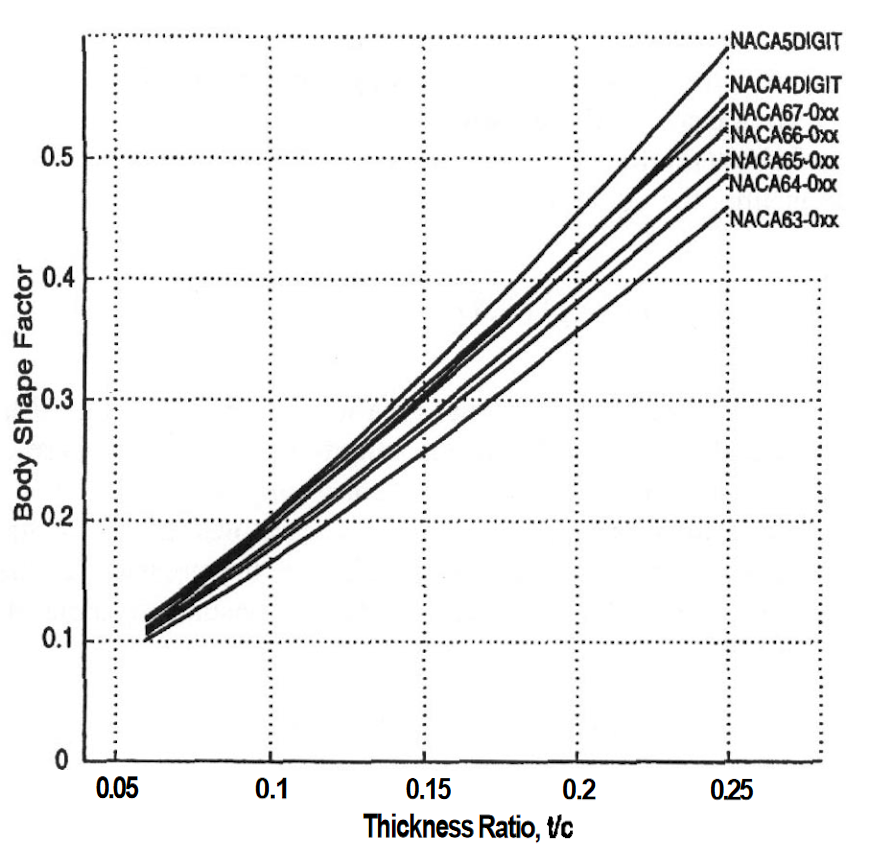
\includegraphics[width=3.5in]{shapeFactor}
    \caption{Body shape factor for common airfoil shapes~\cite{shape}.}
    \label{fig:shape}
\end{figure}

Using Fig.~\ref{fig:shape}, a body shape factor $\Lambda$ of 0.23 was chosen for a NACA 0012 airfoil with a maximum thickness to chord ratio $t/c$ of 0.12.

The next correction accounts for the effect of the wake generated by the object in the test section.
Previous experiments have shown that the mean velocity in the wake region behind an object is lower than the freestream velocity as seen in Fig.~\ref{fig:profile}~\cite{lab3}.

\begin{figure}[H]
    \centering
    % This file was created by matlab2tikz.
%
%The latest updates can be retrieved from
%  http://www.mathworks.com/matlabcentral/fileexchange/22022-matlab2tikz-matlab2tikz
%where you can also make suggestions and rate matlab2tikz.
%
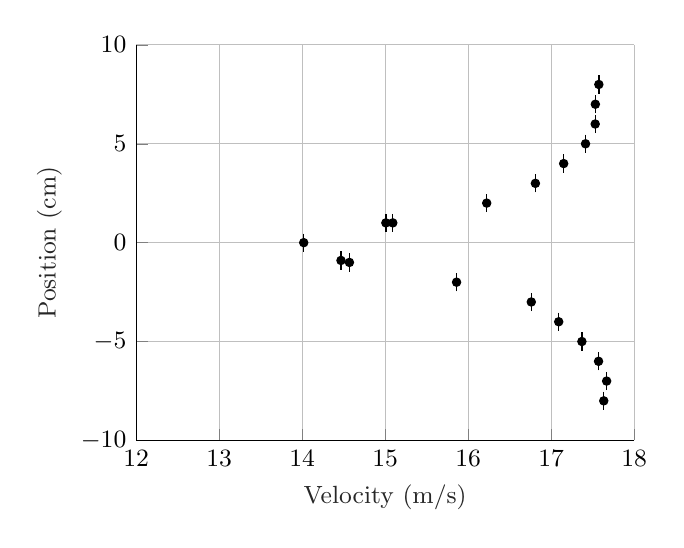
\begin{tikzpicture}

\begin{axis}[%
width=0.958\fwidth,
height=\fheight,
at={(0\fwidth,0\fheight)},
xmin=12,
xmax=18,
xlabel style={font=\color{white!15!black}\small},
xlabel={Velocity (m/s)},
ymin=-10,
ymax=10,
ylabel style={font=\color{white!15!black}\small},
ylabel={Position (cm)},
axis background/.style={fill=white},
axis x line*=bottom,
axis y line*=left,
xmajorgrids,
ymajorgrids,
tick label style={font=\small}
]
\addplot [color=black, only marks, mark size=1.5pt, mark=*, mark options={solid, black}, forget plot]
 plot [error bars/.cd, y dir=both, y explicit, error bar style={line width=0.5pt}, error mark options={line width=0.5pt, mark size=3.0pt, rotate=0}]
 table[row sep=crcr, y error plus index=2, y error minus index=3]{%
17.63302121	-8	0.04	0.04\\
17.66766483	-7	0.04	0.04\\
17.57029602	-6	0.04	0.04\\
17.36951483	-5	0.04	0.04\\
17.09044626	-4	0.04	0.04\\
16.76010295	-3	0.04	0.04\\
15.86014131	-2	0.04	0.04\\
14.5694144	-1	0.04	0.04\\
14.01914389	0	0.04	0.04\\
15.00864139	1	0.04	0.04\\
16.22321569	2	0.04	0.04\\
16.80958078	3	0.04	0.04\\
17.15024428	4	0.04	0.04\\
17.41338612	5	0.04	0.04\\
17.52997475	6	0.04	0.04\\
17.53175424	7	0.04	0.04\\
17.57363723	8	0.04	0.04\\
15.0918459	1	0.04	0.04\\
14.46785862	-0.9	0.04	0.04\\
};
\end{axis}
\end{tikzpicture}%
    \caption{Velocity profile behind a cylinder in uniform flow. This demonstrates the effect of wake blockage~\cite{lab3}.}
    \label{fig:profile}
\end{figure}

The last correction considered in this experiment is accounting for the phenomenon known as streamline curvature.
This occurs because the presence of the ceiling and floor of the test section prevents the normal curvature of the free air due to the lifting body~\cite{lab5r1}.
This has the effect of overestimating the lift, the moment about the quarter chord, and the angle of attack.


\section{Procedure}

\subsection{Gathering Pressure Data Around the Airfoil}

The ambient pressure, relative humidity, and ambient temperature were recorded.
The pressure transducer was calibrated to inches of water in the negative direction using the transducer's digital readout and a water manometer.
The wind tunnel was then set to a relatively high Reynolds number of $241304 \pm 1304$ by using an empty test section and the static gauge pressure difference.
A 4 inch chord length NACA 0012 was then placed into the middle of the test section height-wise as seen in Fig.~\ref{fig:section}.

\begin{figure}[H]
    \centering
    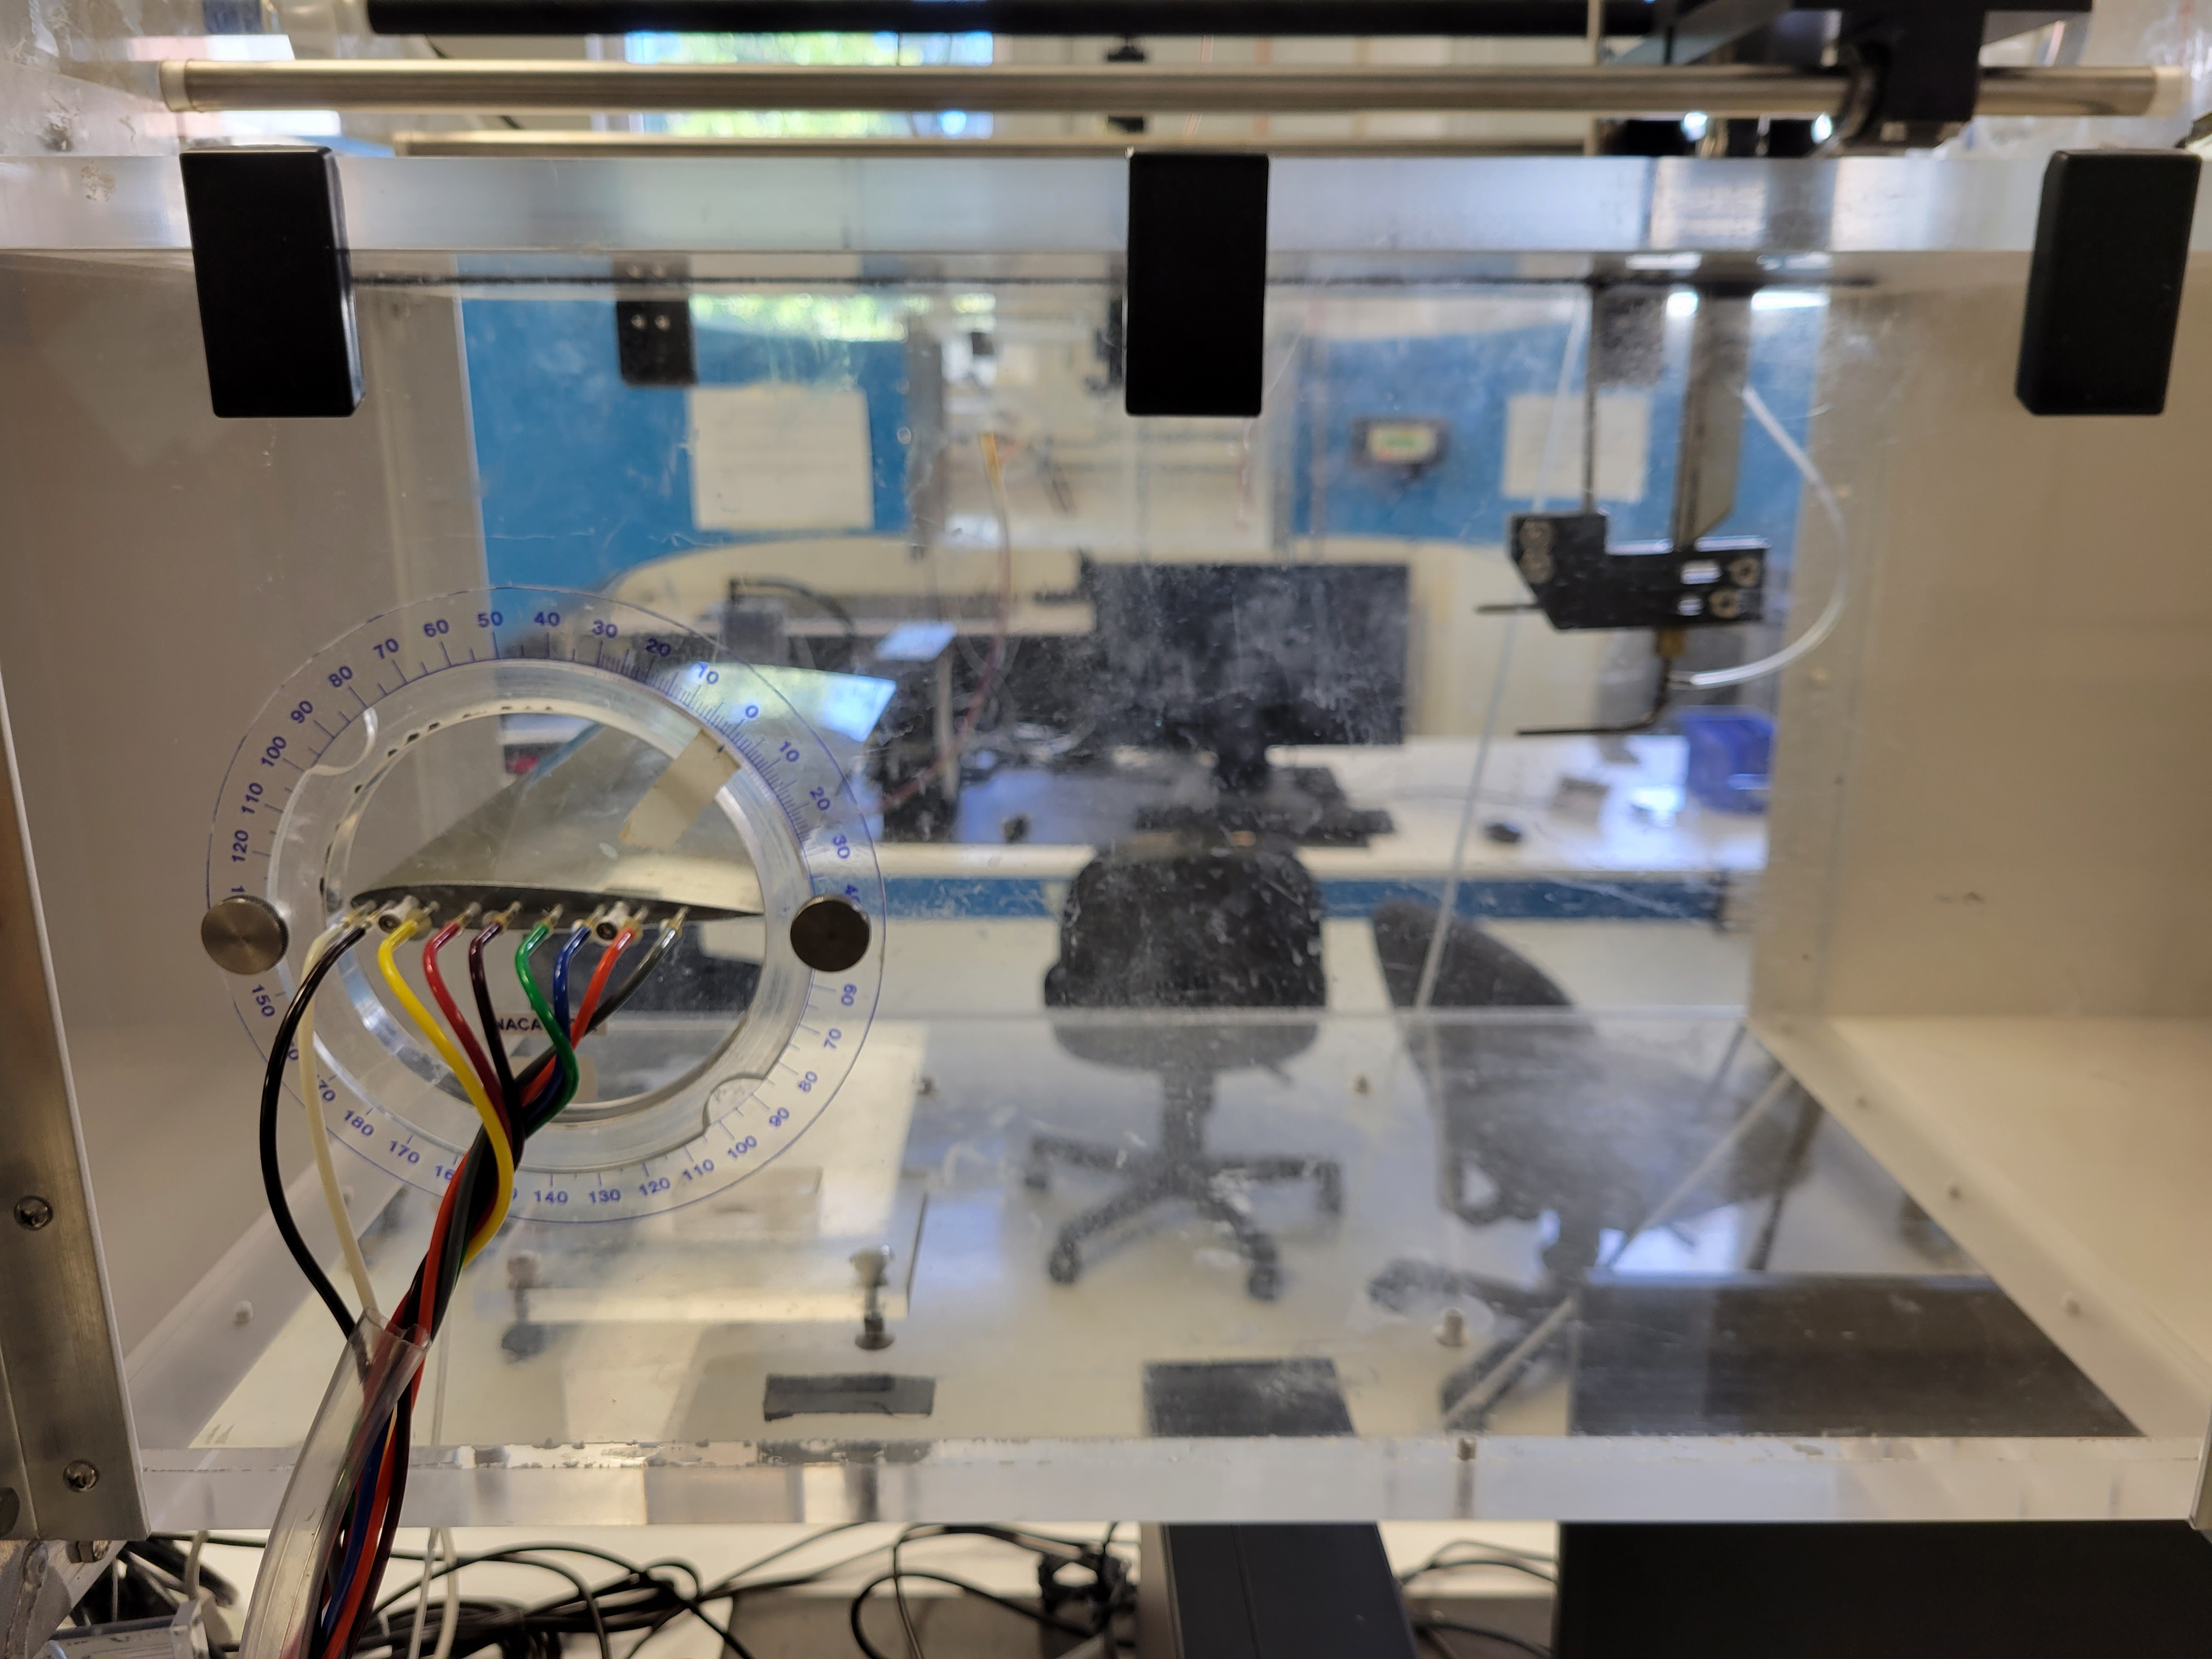
\includegraphics[width=3.5in]{testSection}
    \caption{Wind tunnel test section with NACA 0012 airfoil installed. The airfoil is oriented at an angle of attack of zero degrees.}
    \label{fig:section}
\end{figure}

Starting at an angle of attack of zero degrees and the pre-determined Reynolds number, the static pressure at the nine attached pressure taps were measured at a sampling frequency of \qty{2000}{\Hz} for two seconds each.
The angle of attack was then increased to three degrees, then five degrees, and finally seven degrees.
After seven degrees the angle of attack was increased by one degree until the airfoil was at an angle of attack of thirteen degrees.
For each angle of attack pressure reading, the negative angle of attack was also measured for its nine pressure taps.
This was done at the same sampling rate and time as the previous readings.
As a precaution against signal interference, each time the pressure channel was switched, a wait time of ten seconds was used so that the pressure readings would be accurate.

\subsection{Post-Processing of Pressure Data}

To process the data gathered during the wind tunnel tests, a Python script was used to take the average and calculate the uncertainty of the pressures for all taps at all angles of attack.
The position of each port required for lift and drag calculation was obtained from Fig.~\ref{fig:AirfoilPorts}.
The pressure and length data were then input into a spreadsheet where each pressure was converted into their respective lift and drag forces along with their moments.

\begin{figure}[H]
    \centering
    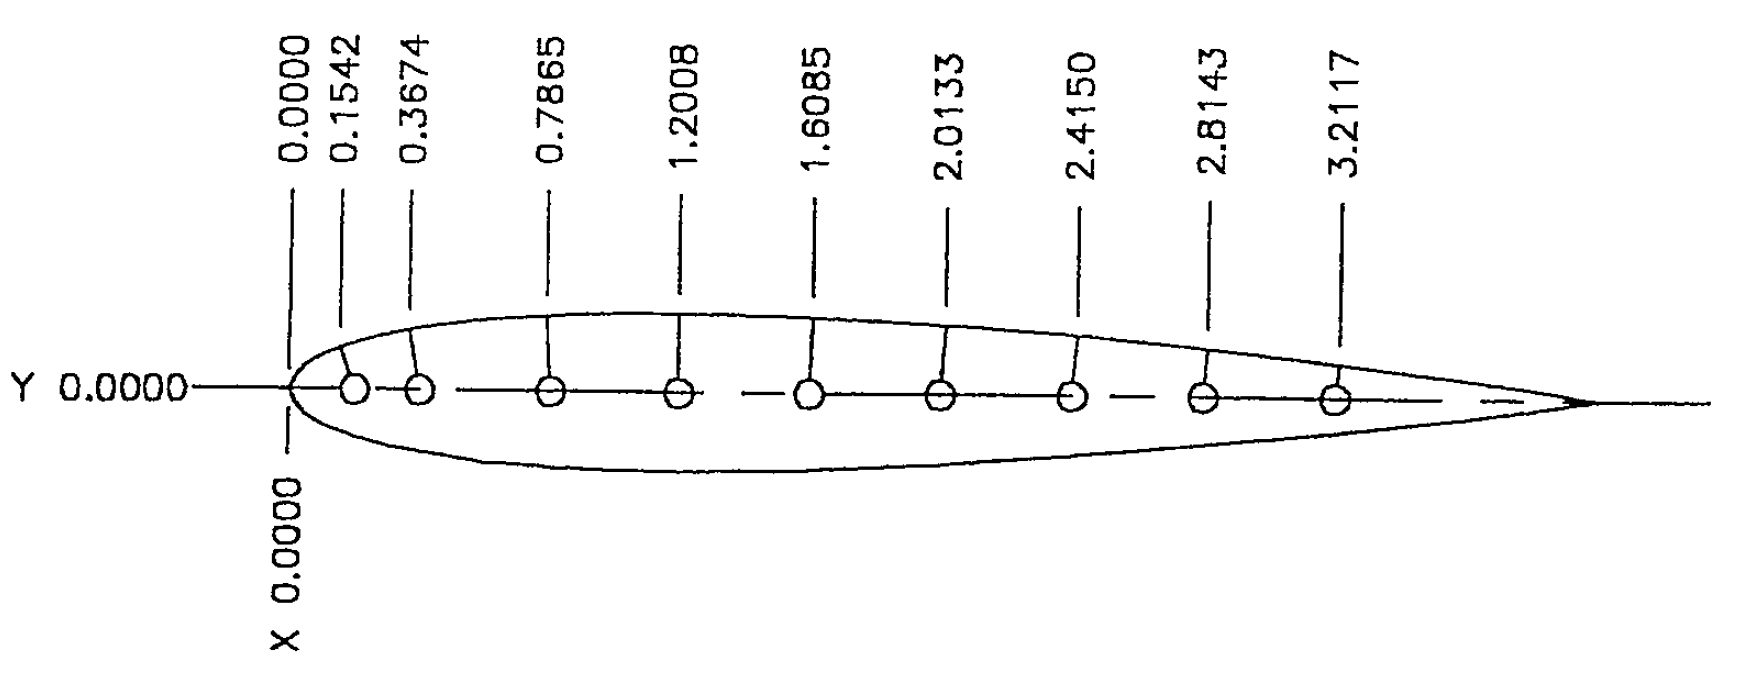
\includegraphics[width=3.5in]{airfoilPorts}
    \caption{Pressure tap locations for the NACA 0012 airfoil used in this experiment. The chord of the airfoil is 4 inches~\cite{ports}.}
    \label{fig:AirfoilPorts}
\end{figure}


\section{Results}


The ambient pressure, $P_\text{amb}$, of the room was measured using a wall-mounted barometer.
The temperature, $T$, and the relative humidity, $\varphi$, of the room was measured using a digital thermometer and hygrometer placed next to the test section.
The measured atmospheric conditions are summarized in Table~\ref{tab:atmCond}.

\begin{table}[H]
    \centering
    \caption{Atmospheric Conditions}
    \renewcommand{\arraystretch}{1.2}
    \begin{tabular}{ccc}
    \toprule
    Parameter & Value & Uncertainty ($\pm$) \\ \midrule \midrule
    $P_\text{amb}$ & \qty{767.70}{mm\ce{Hg}} & \qty{0.02}{mm\ce{Hg}} \\
    $T$ & \qty{21.1}{\celsius} & \qty{0.1}{\celsius} \\
    $\varphi$ & 49\% & 1\% \\ \bottomrule
    \end{tabular}
    \label{tab:atmCond}
\end{table}

The pressures measured around the NACA 0012 airfoil were converted into lift per unit span using the calculated lengths between ports $L^*$, and the pressures measured at the ports.
Each lift value was summed with their negative angle of attack counterpart and plotted against their angle of attack in Fig.~\ref{fig:Lift}.

\begin{figure}[H]
    \centering
    % This file was created by matlab2tikz.
%
%The latest updates can be retrieved from
%  http://www.mathworks.com/matlabcentral/fileexchange/22022-matlab2tikz-matlab2tikz
%where you can also make suggestions and rate matlab2tikz.
%
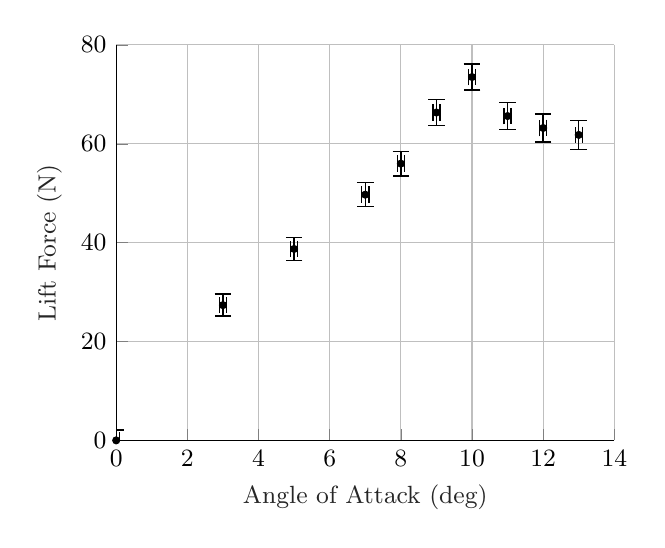
\begin{tikzpicture}

\begin{axis}[%
width=0.958\fwidth,
height=\fheight,
at={(0\fwidth,0\fheight)},
xmin=0,
xmax=14,
xlabel style={font=\color{white!15!black}\small},
xlabel={Angle of Attack (deg)},
ymin=0,
ymax=80,
ylabel style={font=\color{white!15!black}\small},
ylabel={Lift Force (N)},
axis background/.style={fill=white},
axis x line*=bottom,
axis y line*=left,
xmajorgrids,
ymajorgrids,
tick label style={font=\small}
]
\addplot [color=black, only marks, mark size=1.25pt, mark=*, mark options={solid, black}, forget plot]
 plot [error bars/.cd, x dir=both, x explicit, y dir=both, y explicit, error bar style={line width=0.5pt}, error mark options={line width=0.5pt, mark size=3.0pt, rotate=90}]
 table[row sep=crcr, y error index=2, x error index=3]{%
0	0	2.1	0.1\\
3	27.35742964	2.22	0.1\\
5	38.72684467	2.31	0.1\\
7	49.70505638	2.45	0.1\\
8	55.98542969	2.5	0.1\\
9	66.32375174	2.58	0.1\\
10	73.4976954	2.61	0.1\\
11	65.60831974	2.75	0.1\\
12	63.19365752	2.85	0.1\\
13	61.79559985	2.96	0.1\\
};
\end{axis}
\end{tikzpicture}%
    \caption{Lift force versus angle of attack for NACA 0012 airfoil.}
    \label{fig:Lift}
\end{figure}

The pressures measured at the pressure taps were then converted into their respective drag forces at each angle of attack using the same method as the lift.
The drag forces were then plotted against their angle of attack in Fig.~\ref{fig:Drag}.

\begin{figure}[H]
    \centering
    % This file was created by matlab2tikz.
%
%The latest updates can be retrieved from
%  http://www.mathworks.com/matlabcentral/fileexchange/22022-matlab2tikz-matlab2tikz
%where you can also make suggestions and rate matlab2tikz.
%
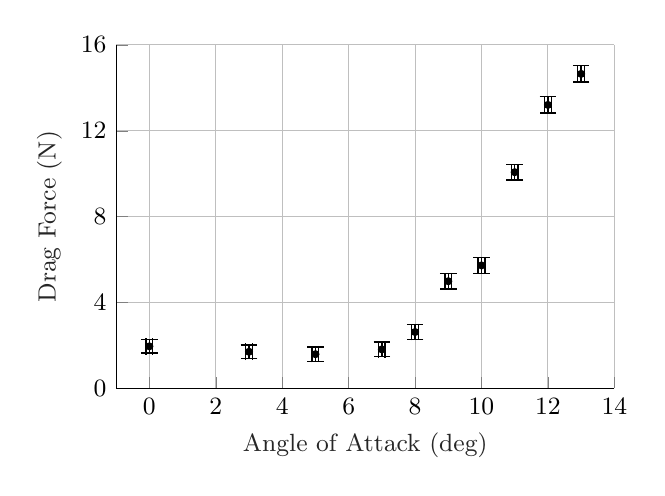
\begin{tikzpicture}

\begin{axis}[%
width=0.958\fwidth,
height=0.9\fheight,
at={(0\fwidth,0\fheight)},
xmin=-1,
xmax=14,
xlabel style={font=\color{white!15!black}\small},
xlabel={Angle of Attack (deg)},
ymin=0,
ymax=16,
ylabel style={font=\color{white!15!black}\small},
ylabel={Drag Force (N)},
ytick={0,4,...,16},
axis background/.style={fill=white},
axis x line*=bottom,
axis y line*=left,
xmajorgrids,
ymajorgrids,
tick label style={font=\small}
]
\addplot [color=black, only marks, mark size=1.25pt, mark=*, mark options={solid, black}, forget plot]
plot [error bars/.cd, x dir=both, x explicit, y dir=both, y explicit, error bar style={line width=0.5pt}, error mark options={line width=0.5pt, mark size=3.0pt, rotate=90}]
table[row sep=crcr, y error index=2, x error index=3]{%
0	1.958206345	0.312	0.1\\
3	1.704549533	0.324	0.1\\
5	1.592962649	0.339	0.1\\
7	1.817184317	0.343	0.1\\
8	2.625310249	0.355	0.1\\
9	4.99126022	0.361	0.1\\
10	5.728481418	0.369	0.1\\
11	10.07077517	0.372	0.1\\
12	13.20591133	0.379	0.1\\
13	14.65105534	0.384	0.1\\
};
\end{axis}
\end{tikzpicture}%
    \caption{Drag force versus angle of attack for NACA 0012 airfoil.}
    \label{fig:Drag}
\end{figure}

Using the lifts and drags generated, the moments of the airfoil's quarter chord can then be calculated and plotted against their respective angles of attack in Fig.~\ref{fig:Moment}.

\begin{figure}[H]
    \centering
    % This file was created by matlab2tikz.
%
%The latest updates can be retrieved from
%  http://www.mathworks.com/matlabcentral/fileexchange/22022-matlab2tikz-matlab2tikz
%where you can also make suggestions and rate matlab2tikz.
%
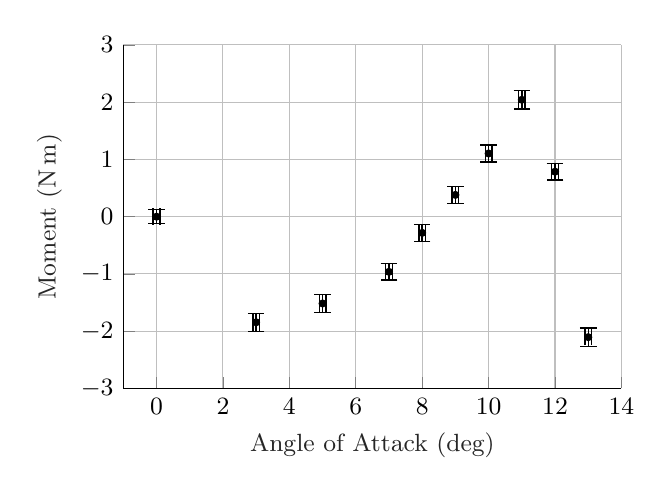
\begin{tikzpicture}

\begin{axis}[%
width=0.958\fwidth,
height=0.9\fheight,
at={(0\fwidth,0\fheight)},
xmin=-1,
xmax=14,
xlabel style={font=\color{white!15!black}\small},
xlabel={Angle of Attack (deg)},
ymin=-3,
ymax=3,
ylabel style={font=\color{white!15!black}\small},
ylabel={Moment (\unit{\newton\meter})},
ytick={-3,-2,...,3},
axis background/.style={fill=white},
axis x line*=bottom,
axis y line*=left,
xmajorgrids,
ymajorgrids,
tick label style={font=\small}
]
\addplot [color=black, only marks, mark size=1.25pt, mark=*, mark options={solid, black}, forget plot]
plot [error bars/.cd, x dir=both, x explicit, y dir=both, y explicit, error bar style={line width=0.5pt}, error mark options={line width=0.5pt, mark size=3.0pt, rotate=90}]
table[row sep=crcr, y error index=2, x error index=3]{%
0	0	0.121	0.1\\
3	-1.845242185	0.158	0.1\\
5	-1.516790206	0.153	0.1\\
7	-0.9641498	0.144	0.1\\
8	-0.283300244	0.146	0.1\\
9	0.37970687	0.145	0.1\\
10	1.103431109	0.15	0.1\\
11	2.041708102	0.16	0.1\\
12	0.785569658	0.148	0.1\\
13	-2.105218776	0.161	0.1\\
};
\end{axis}
\end{tikzpicture}%
    \caption{Moment about the quarter chord versus angle of attack for NACA 0012 airfoil.}
    \label{fig:Moment}
\end{figure}


\section{Discussion}

\subsection{Pressure Data Disclaimer}

One important consideration is that the pressure port 1 on the airfoil was found to be blocked with debris, which gave inconsistent readings for the static pressure.
This in turn affected all data coming from the pressure calculations.
To remedy this, the pressure at port 1 was assumed to be the same as the pressure measured at port 2.
This will allow an approximation of the lift, drag, and moment data.
The effects of this approximation are an increase in drag, a decrease in calculated lift, and a decrease in the calculated moments.

\subsection{Aerodynamic Coefficients Calculation}

To calculate the lift and drag, the position of each port on the airfoil must be known.
The $y$-location of each port was determined using~\eqref{eq:airfoil}, where $x$ is the horizontal location of the pressure port given in Fig.~\ref{fig:AirfoilPorts} and $t$ is the maximum thickness of the airfoil as a fraction of the chord~\cite{AirfoilEq}.

\begin{equation} \label{eq:airfoil}
    \resizebox{227pt}{!}{$\displaystyle{\pm y = 5t(0.2969\sqrt{x} - 0.126x - 0.3516x^2 + 0.2843x^3 - 0.1015x^4)}$}
\end{equation}

The maximum thickness $t$ is determined by dividing the last two digits of the four-digit denomination by 100~\cite{AirfoilEq}.
For the NACA 0012, the maximum thickness is 12\% of the chord.
Before calculating the $y$-location for each port, the $x$-location was normalized by dividing by chord length.
This yields the normalized $y$-location of each port, which can be multiplied by the chord length to find the actual $y$-location.

To find the lift and drag coefficients, the pressure distribution over the surface of the airfoil must be integrated.
Since pressure was measured at discrete points, the line integral for lift and drag was computed numerically using line integration.
To do this, the length $L_i^*$ that a specific pressure acts over is required, where $i$ is the port number.
This is determined by obtaining the horizontal distance $\Delta x_i$ and the vertical distance $\Delta y_i$ between the ports.
A method similar to a midpoint integration scheme was used to find these values.
For example, when calculating $\Delta x_i$ for the line that the pressure measured by port 2 acts over, the distance between the midpoint between ports 1 and 2 and the midpoint between ports 2 and 3 was used.
For ports 1 and 9, the line was extended to meet the leading edge and trailing edge of the airfoil, respectively.
Next,~\eqref{eq:airfoil} can be used to calculate the $y$ locations of each port. Then, the vertical distance $\Delta y_i$ was calculated using a similar method to $\Delta x_i$. Using these values, $L_i^*$ is computed using~\eqref{eq:Lstar}.
\begin{equation} \label{eq:Lstar}
    L_i^* = \sqrt{\left(\Delta x_i\right)^2 + \left(\Delta y_i\right)^2}
\end{equation}
The angle of the line that the pressure at a specific port acts over can now be calculated using~\eqref{eq:Theta}, where $\theta_i$ is the angle between the centerline of the airfoil and the line that the pressure measured at port $i$ acts.
\begin{equation} \label{eq:Theta}
    \theta_i = \arctan\left(\frac{\Delta y_i}{\Delta x_i}\right)
\end{equation}
Next, using~\eqref{eq:Gamma}, the angle $\gamma_i$ between the line that the pressure at port $i$ acts and the freestream is computed.
\begin{equation} \label{eq:Gamma}
    \gamma_i = \theta_i - \alpha
\end{equation}
Using these calculations, the lift forces $L'_i$ and drag forces $D'_i$  per unit span for each port $i$ can be calculated using~\eqref{eq:LiftF} and~\eqref{eq:DragF}.
\begin{equation} \label{eq:LiftF}
    L'_i = P_i L_i^* \cos\left(\gamma_i\right)
\end{equation}

\begin{equation} \label{eq:DragF}
    D'_i = P_i L_i^* \sin\left(\gamma_i\right)
\end{equation}
These calculated lift and drag forces are then summed for all ports at a specific angle of attack.
Then, the positive angles of attack were combined with the same negative angles of attack.
This is possible because the airfoil is symmetric and there are no ports on the bottom of the airfoil.

The moments at a specific port were calculated using~\eqref{eq:Moment}, where $M_i$ is the moment at port $i$, $x_i$ is the horizontal location of port $i$, $y_i$ is the horizontal location of port $i$, and $c$ is the chord length of the airfoil. The moments were taken about the quarter chord location.
\begin{equation} \label{eq:Moment}
    M_i = L'_i\left(x_i - \frac{c}{4}\right) + D'_iy_i
\end{equation}

The coefficients of these values are calculated using~\eqref{eq:CL},~\eqref{eq:CD}, and~\eqref{eq:CM}, where $q$ is the dynamic pressure and $c$ is the chord of the airfoil.
\begin{equation} \label{eq:CL}
    C_L = \frac{L'}{qc}
\end{equation}

\begin{equation} \label{eq:CD}
    C_D = \frac{D'}{qc}
\end{equation}

\begin{equation} \label{eq:CM}
    C_M = \frac{M}{qc^2}
\end{equation}

\subsection{Wind Tunnel Correction}

The XFLR5 software generates the flight characteristics of the NACA 0012 airfoil by assuming it is in an unbounded free stream.
The experimental data was performed in the test section of a wind tunnel which causes performance deviation from the free stream assumption due to factors such as solid blockage, wake blockage, and streamline curvature.
To account for these deviations, the following corrections were made to the data.

Previous experimentation has suggested that the percent speed increase for flow outside of the wake boundary due to an airfoil, $\varepsilon_{wb}$, can be estimated by~\eqref{eq:wb}, where $c$ is the chord length, $h$ is the tunnel height, and $C_{Du}$ is the uncorrected drag coefficient~\cite{lab5r1}.
\begin{equation} \label{eq:wb}
    \varepsilon_{wb} = \frac{c/h}{2}C_{Du}
\end{equation}
Then, it is useful to define the total percent velocity increase due to solid blockage and wake blockage as $\varepsilon$, where $\varepsilon_{sb}$ is the percent velocity increase due to solid blockage and $\varepsilon_{wb}$ is the percent velocity increase due to wake blockage as seen in~\eqref{eq:ep}.
\begin{equation} \label{eq:ep}
    \varepsilon = \varepsilon_{sb} + \varepsilon_{wb}
\end{equation}
The freestream velocity ($U_\infty$), Reynolds number ($Re$), and dynamic pressure ($q$), can then be corrected with~\eqref{eq:Vu},~\eqref{eq:Reu}, and~\eqref{eq:qu} respectively, where a subscript of $u$ denotes the uncorrected corresponding value.
\begin{equation} \label{eq:Vu}
    U_\infty = U_{\infty u}(1 + \varepsilon)
\end{equation}

\begin{equation} \label{eq:Reu}
    Re = Re_u(1 + \varepsilon)
\end{equation}

\begin{equation} \label{eq:qu}
    q = q_u(1 + \varepsilon)
\end{equation}
To account for the deviations in the aerodynamic force coefficients and the angle of attack, it is useful to define the wind-tunnel correction parameter, $\sigma$, with~\eqref{eq:sigma} where $c$ is the chord length and $h$ is the height of the test section.
\begin{equation} \label{eq:sigma}
    \sigma = \left(\frac{\pi^2}{48}\right)\left(\frac{c}{h}\right)^2
\end{equation}
The angle of attack $\alpha$, coefficient of lift $C_L$, coefficient of drag $C_D$, and the moment coefficient about the quarter chord $C_{M\frac{1}{4}}$ can all be corrected with~\eqref{eq:alphau},~\eqref{eq:liftu},~\eqref{eq:dragu}, and~\eqref{eq:Mu} respectively where a subscript of $u$ notes the uncorrected value.
\begin{equation} \label{eq:alphau}
    \alpha = \alpha_u + \frac{57.3\sigma}{2\pi} \left(C_{Lu} + 4C_{M\frac{1}{4}}\right)
\end{equation}

\begin{equation} \label{eq:liftu}
    C_L = C_{Lu} (1 - \sigma - 2\varepsilon)
\end{equation}

\begin{equation} \label{eq:dragu}
    C_D = C_{Du} (1 - 3\varepsilon_{sb} - 2\varepsilon_{wb})
\end{equation}

\begin{equation} \label{eq:Mu}
    C_{M\frac{1}{4}} = C_{M\frac{1}{4}u} (1 - 2\varepsilon) + \frac{1}{4}\sigma C_L  
\end{equation}

\subsection{XFLR5 Simulation of NACA 0012 Airfoil}

To obtain theoretical data for the flight performance of the NACA 0012 airfoil, the XFLR5 version 6.56 analysis tool was used.
While the original instructions were to use the XFOIL software, the team decided to opt for XFLR5 for its enhanced graphical user interface, familiarity with the software, and the fact that XFLR5 runs the XFOIL software in the background when performing calculations on 2D airfoils.
This substitution was deemed acceptable by the instructors.

To obtain the theoretical lift, drag, and moment polars, the 2D airfoil simulation was run at the same range of angle of attacks as the uncorrected data and at the same corrected Reynolds number of $241304 \pm 1304$ as in the experiment.

\subsection{Comparison of Uncorrected, Corrected, and Theoretical Coefficients}

For each of the lift, drag, and moment polars, the following sets of data were plotted: the uncorrected experimental data, the corrected experimental data, and the theoretical airfoil data from XFLR5.
As can be seen in Fig.~\ref{fig:complift}, the uncorrected data aligned closer to the theoretical XFLR5 data than the original corrected data.
However, the corrected data was found to be closer to the XFLR5 data for the drag and moment polars as seen in Fig.~\ref{fig:compdrag} and Fig.~\ref{fig:compmoment}. 

\begin{figure}[H]
    \centering
    % This file was created by matlab2tikz.
%
%The latest updates can be retrieved from
%  http://www.mathworks.com/matlabcentral/fileexchange/22022-matlab2tikz-matlab2tikz
%where you can also make suggestions and rate matlab2tikz.
%
\definecolor{mycolor1}{rgb}{0.00000,0.44700,0.74100}%
\definecolor{mycolor2}{rgb}{0.98039,0.27451,0.08627}%
\definecolor{mycolor3}{rgb}{0.85000,0.32500,0.09800}%
\definecolor{mycolor4}{rgb}{0.00000,0.12941,0.64706}%
%
\begin{tikzpicture}

\begin{axis}[%
width=0.958\fwidth,
height=\fheight,
at={(0\fwidth,0\fheight)},
xmin=-2,
xmax=14,
xlabel style={font=\color{white!15!black}\small},
xlabel={Angle of Attack (deg)},
ymin=-0.2,
ymax=1.2,
yticklabel style={
            /pgf/number format/fixed,
            /pgf/number format/precision=1,
            /pgf/number format/fixed zerofill
        },
ylabel style={font=\color{white!15!black}\small},
ylabel={$C_L$},
ytick={-0.2,0,...,1.2},
axis background/.style={fill=white},
axis x line*=bottom,
axis y line*=left,
xmajorgrids,
ymajorgrids,
tick label style={font=\small},
legend style={at={(0.03,0.97)}, anchor=north west, legend cell align=left, align=left, draw=white!15!black, font=\footnotesize}
]
\addplot [color=black, only marks, mark=triangle*, mark options={solid, fill=mycolor2, draw=mycolor2}]
plot [error bars/.cd, x dir=both, x explicit, y dir=both, y explicit, error bar style={line width=0.5pt}, error mark options={line width=0.5pt, mark size=3.0pt, rotate=90}]
table[row sep=crcr, y error index=2, x error index=3]{%
0	0	0.03	0.1\\
3	0.336668611	0.034	0.1\\
5	0.476583991	0.039	0.1\\
7	0.611685107	0.043	0.1\\
8	0.688973236	0.048	0.1\\
9	0.816199681	0.052	0.1\\
10	0.904484351	0.057	0.1\\
11	0.807395364	0.061	0.1\\
12	0.777679817	0.066	0.1\\
13	0.760474906	0.07	0.1\\
};
\addlegendentry{Uncorrected}

\addplot [color=black, only marks, mark=square*, mark options={solid, fill=mycolor4, draw=mycolor4}]
plot [error bars/.cd, x dir=both, x explicit, y dir=both, y explicit, error bar style={line width=0.5pt}, error mark options={line width=0.5pt, mark size=3.0pt, rotate=90}]
table[row sep=crcr, y error index=2, x error index=3]{%
0	0	0.03	0.1\\
3.051219576	0.32308476	0.034	0.1\\
5.083739423	0.457573009	0.039	0.1\\
7.117555465	0.586722313	0.043	0.1\\
8.140641138	0.658572369	0.048	0.1\\
9.173948407	0.77226345	0.052	0.1\\
10.19552088	0.853060434	0.057	0.1\\
11.17868962	0.74710964	0.061	0.1\\
12.17634195	0.709611403	0.066	0.1\\
13.1769283	0.689404208	0.07	0.1\\
};
\addlegendentry{Corrected}

\addplot [color=black, line width=1.2pt]
  table[row sep=crcr]{%
0	7.591131e-08\\
0.05	0.006087696\\
0.1	0.01068031\\
0.15	0.01644907\\
0.2	0.02266503\\
0.25	0.0279591\\
0.3	0.03285344\\
0.35	0.03937355\\
0.4	0.04534203\\
0.45	0.05044477\\
0.5	0.05611996\\
0.55	0.06271658\\
0.6	0.06883336\\
0.65	0.07432752\\
0.7	0.08002458\\
0.75	0.08698604\\
0.8	0.09377797\\
0.85	0.09974366\\
0.9	0.1049151\\
1	0.1198396\\
1.05	0.1268369\\
1.1	0.1329461\\
1.15	0.1390644\\
1.2	0.1470974\\
1.25	0.1549672\\
1.3	0.1625394\\
1.35	0.1694755\\
1.4	0.1752715\\
1.45	0.1837845\\
1.5	0.1923523\\
1.55	0.2008495\\
1.6	0.2091159\\
1.65	0.2167416\\
1.7	0.22285\\
1.75	0.2319172\\
1.8	0.2406811\\
1.85	0.2493365\\
1.9	0.257542\\
1.95	0.26536\\
2	0.2717372\\
2.05	0.2805552\\
2.1	0.2892318\\
2.15	0.2977933\\
2.2	0.3059277\\
2.25	0.3136488\\
2.3	0.3208306\\
2.35	0.3296854\\
2.4	0.3382555\\
2.45	0.3466762\\
2.5	0.3546684\\
2.55	0.3622963\\
2.6	0.3707761\\
2.65	0.3794834\\
2.7	0.3878211\\
2.75	0.3961511\\
2.8	0.4040956\\
2.85	0.412788\\
2.9	0.4213241\\
2.95	0.4297763\\
3	0.4382094\\
3.05	0.4466675\\
3.1	0.4553052\\
3.15	0.4635318\\
3.2	0.4681316\\
3.25	0.4726614\\
3.3	0.4772745\\
3.35	0.481783\\
3.4	0.4864077\\
3.5	0.495531\\
3.55	0.5000216\\
3.6	0.5046334\\
3.65	0.5091103\\
3.7	0.5137123\\
3.75	0.5181746\\
3.8	0.5227605\\
3.85	0.5271939\\
3.9	0.5317627\\
4	0.5407129\\
4.05	0.5450685\\
4.1	0.5495853\\
4.15	0.5539042\\
4.2	0.55834\\
4.25	0.5626258\\
4.3	0.567002\\
4.35	0.5712918\\
4.4	0.5756076\\
4.45	0.5799055\\
4.5	0.5841506\\
4.55	0.5884604\\
4.6	0.5926261\\
4.65	0.5969503\\
4.7	0.6010611\\
4.75	0.6053616\\
4.8	0.6095006\\
4.85	0.6136901\\
4.9	0.6178609\\
4.95	0.6219378\\
5	0.6261431\\
5.05	0.6301258\\
5.1	0.6343411\\
5.15	0.63836\\
5.2	0.6424503\\
5.25	0.6465056\\
5.3	0.6504786\\
5.35	0.6545705\\
5.4	0.6584417\\
5.45	0.6625686\\
5.55	0.6705097\\
5.6	0.6742702\\
5.65	0.6783998\\
5.75	0.6862439\\
5.8	0.6899846\\
5.85	0.6940365\\
5.9	0.6978597\\
5.95	0.7017296\\
6	0.7056933\\
6.05	0.7092564\\
6.1	0.7134061\\
6.15	0.7172303\\
6.2	0.7208399\\
6.25	0.7249693\\
6.3	0.7287518\\
6.35	0.7322772\\
6.4	0.7364352\\
6.45	0.7403047\\
6.5	0.7437605\\
6.55	0.7477439\\
6.6	0.7517475\\
6.65	0.7555262\\
6.7	0.7588181\\
6.75	0.7629576\\
6.8	0.7669733\\
6.85	0.7708114\\
6.9	0.7742407\\
6.95	0.7779873\\
7	0.7820981\\
7.05	0.7860279\\
7.1	0.7897944\\
7.15	0.7931705\\
7.2	0.7968178\\
7.25	0.800914\\
7.3	0.80485\\
7.35	0.8086865\\
7.4	0.812358\\
7.45	0.8156253\\
7.5	0.8193537\\
7.55	0.8234845\\
7.6	0.8274684\\
7.65	0.831359\\
7.7	0.8351497\\
7.75	0.8387385\\
7.8	0.8418624\\
7.85	0.8460191\\
7.9	0.8501353\\
7.95	0.8541358\\
8	0.858068\\
8.05	0.8619393\\
8.1	0.8657253\\
8.15	0.8693408\\
8.2	0.8726584\\
8.25	0.8766557\\
8.3	0.8807976\\
8.35	0.8848596\\
8.4	0.8888785\\
8.45	0.8928684\\
8.5	0.896825\\
8.55	0.900733\\
8.6	0.9045538\\
8.65	0.9082116\\
8.7	0.9119297\\
8.75	0.9160518\\
8.8	0.9201116\\
8.85	0.9241391\\
8.9	0.9281468\\
8.95	0.9321429\\
9	0.9361314\\
9.05	0.9401115\\
9.1	0.9440701\\
9.15	0.9480146\\
9.2	0.9519454\\
9.25	0.9558778\\
9.3	0.9597999\\
9.35	0.9637297\\
9.4	0.9676648\\
9.45	0.9716031\\
9.5	0.9755011\\
9.55	0.9793952\\
9.6	0.9832962\\
9.65	0.9872172\\
9.7	0.9911573\\
9.75	0.9951245\\
9.8	0.9991384\\
9.85	1.003231\\
9.9	1.007433\\
9.95	1.01159\\
10	1.014827\\
10.05	1.018142\\
10.1	1.021526\\
10.15	1.024967\\
10.2	1.028461\\
10.25	1.032007\\
10.3	1.03558\\
10.35	1.039088\\
10.4	1.042625\\
10.45	1.046185\\
10.5	1.049778\\
10.55	1.05346\\
10.6	1.05722\\
10.65	1.06108\\
10.7	1.065083\\
10.75	1.069287\\
10.8	1.073704\\
10.85	1.076087\\
10.9	1.078299\\
10.95	1.080522\\
11	1.082745\\
11.05	1.084952\\
11.1	1.087133\\
11.15	1.089291\\
11.2	1.09142\\
11.25	1.093521\\
11.3	1.095605\\
11.35	1.097689\\
11.4	1.099792\\
11.45	1.101937\\
11.5	1.104149\\
11.55	1.106466\\
11.6	1.108922\\
11.65	1.111555\\
11.7	1.113894\\
11.75	1.116173\\
11.8	1.118536\\
11.85	1.12098\\
11.9	1.123518\\
11.95	1.126279\\
12	1.129483\\
12.05	1.132691\\
12.1	1.134402\\
12.15	1.132967\\
12.2	1.131123\\
12.25	1.129039\\
12.3	1.126869\\
12.35	1.124652\\
12.4	1.1224\\
12.45	1.120123\\
12.5	1.117837\\
12.55	1.115529\\
12.6	1.11318\\
12.65	1.110778\\
12.7	1.108306\\
12.75	1.10576\\
12.8	1.103122\\
12.85	1.100386\\
12.9	1.097548\\
12.95	1.094594\\
13	1.091521\\
};
\addlegendentry{XFLR5}

\end{axis}
\end{tikzpicture}%
    \caption{Uncorrected (orange triangle) and corrected (blue square) coeffiecent of lift versus angle of attack. The data from XFLR5 is plotted as a solid black line.}
    \label{fig:complift}
\end{figure}

\begin{figure}[H]
    \centering
    % This file was created by matlab2tikz.
%
%The latest updates can be retrieved from
%  http://www.mathworks.com/matlabcentral/fileexchange/22022-matlab2tikz-matlab2tikz
%where you can also make suggestions and rate matlab2tikz.
%
\definecolor{mycolor1}{rgb}{0.00000,0.44700,0.74100}%
\definecolor{mycolor2}{rgb}{0.98039,0.27451,0.08627}%
\definecolor{mycolor3}{rgb}{0.85000,0.32500,0.09800}%
\definecolor{mycolor4}{rgb}{0.00000,0.12941,0.64706}%
%
\begin{tikzpicture}

\begin{axis}[%
width=0.958\fwidth,
height=\fheight,
at={(0\fwidth,0\fheight)},
xmin=-2,
xmax=14,
xlabel style={font=\color{white!15!black}\small},
xlabel={Angle of Attack (deg)},
ymin=-0.05,
ymax=0.25,
yticklabel style={
            /pgf/number format/fixed,
            /pgf/number format/precision=2,
            /pgf/number format/fixed zerofill
        },
ylabel style={font=\color{white!15!black}\small},
ylabel={$C_D$},
ytick={-0.05,0,...,0.25},
axis background/.style={fill=white},
axis x line*=bottom,
axis y line*=left,
xmajorgrids,
ymajorgrids,
tick label style={font=\small},
legend style={at={(0.03,0.97)}, anchor=north west, legend cell align=left, align=left, draw=white!15!black, font=\footnotesize}
]
\addplot [color=black, only marks, mark=triangle*, mark options={solid, fill=mycolor2, draw=mycolor2}]
plot [error bars/.cd, x dir=both, x explicit, y dir=both, y explicit, error bar style={line width=0.5pt}, error mark options={line width=0.5pt, mark size=3.0pt, rotate=90}]
table[row sep=crcr, y error index=2, x error index=3]{%
0	0.024098266	0.01	0.1\\
3	0.02097669	0.012	0.1\\
5	0.019603469	0.014	0.1\\
7	0.022362807	0.017	0.1\\
8	0.032307843	0.019	0.1\\
9	0.061423923	0.021	0.1\\
10	0.070496385	0.023	0.1\\
11	0.123933934	0.026	0.1\\
12	0.162515846	0.028	0.1\\
13	0.180300215	0.03	0.1\\
};
\addlegendentry{Uncorrected}

\addplot [color=black, only marks, mark=square*, mark options={solid, fill=mycolor4, draw=mycolor4}]
plot [error bars/.cd, x dir=both, x explicit, y dir=both, y explicit, error bar style={line width=0.5pt}, error mark options={line width=0.5pt, mark size=3.0pt, rotate=90}]
table[row sep=crcr, y error index=2, x error index=3]{%
0	0.023524806	0.01	0.1\\
3.051219576	0.020477514	0.012	0.1\\
5.083739423	0.019136971	0.014	0.1\\
7.117555465	0.021830646	0.017	0.1\\
8.140641138	0.031539023	0.019	0.1\\
9.173948407	0.059962236	0.021	0.1\\
10.19552088	0.068818803	0.023	0.1\\
11.17868962	0.120984715	0.026	0.1\\
12.17634195	0.158648504	0.028	0.1\\
13.1769283	0.176009664	0.03	0.1\\
};
\addlegendentry{Corrected}

\addplot [color=black, line width=1.2pt]
  table[row sep=crcr]{%
0	0.008842244\\
0.05	0.008839894\\
0.1	0.008842193\\
0.15	0.008848226\\
0.2	0.008853654\\
0.25	0.008862198\\
0.3	0.008866107\\
0.35	0.008878755\\
0.4	0.008894147\\
0.45	0.008904845\\
0.5	0.008914627\\
0.55	0.008936335\\
0.6	0.008956403\\
0.65	0.008970107\\
0.7	0.008987954\\
0.75	0.009013733\\
0.8	0.009038003\\
0.85	0.009060692\\
0.9	0.009078774\\
1	0.009138079\\
1.05	0.009166962\\
1.1	0.009193608\\
1.15	0.009218441\\
1.2	0.009252837\\
1.25	0.009284323\\
1.3	0.009317042\\
1.35	0.009349723\\
1.4	0.009375954\\
1.45	0.009413921\\
1.5	0.009445401\\
1.55	0.0094814\\
1.6	0.009514411\\
1.65	0.009547555\\
1.7	0.009583161\\
1.75	0.009614014\\
1.8	0.009653574\\
1.85	0.009682475\\
1.9	0.009723635\\
1.95	0.009752705\\
2	0.00979463\\
2.05	0.009823753\\
2.1	0.00986176\\
2.15	0.009892156\\
2.2	0.009931544\\
2.25	0.009964881\\
2.3	0.01000745\\
2.35	0.01003672\\
2.4	0.01007481\\
2.45	0.01010592\\
2.5	0.01014927\\
2.55	0.01018592\\
2.6	0.01022726\\
2.65	0.01025297\\
2.7	0.01029726\\
2.75	0.01032646\\
2.8	0.01037541\\
2.85	0.01040184\\
2.9	0.01043647\\
2.95	0.01047335\\
3	0.01051069\\
3.05	0.01055327\\
3.1	0.01057927\\
3.15	0.0106249\\
3.2	0.01064561\\
3.25	0.01068194\\
3.3	0.01070268\\
3.35	0.01074377\\
3.4	0.01076468\\
3.5	0.01083134\\
3.55	0.01087682\\
3.6	0.01090314\\
3.65	0.01095069\\
3.7	0.01097975\\
3.75	0.01102941\\
3.8	0.01106126\\
3.85	0.01111418\\
3.9	0.0111482\\
4	0.01124038\\
4.05	0.01130053\\
4.1	0.01133826\\
4.15	0.01139919\\
4.2	0.0114428\\
4.25	0.01150394\\
4.3	0.0115539\\
4.35	0.01161466\\
4.4	0.01167191\\
4.45	0.01173192\\
4.5	0.01179726\\
4.55	0.01185614\\
4.6	0.0119304\\
4.65	0.01198779\\
4.7	0.01206803\\
4.75	0.01212793\\
4.8	0.01220521\\
4.85	0.01227707\\
4.9	0.01235131\\
4.95	0.01243529\\
5	0.01250634\\
5.05	0.01260047\\
5.1	0.01267079\\
5.15	0.01276157\\
5.2	0.01284501\\
5.25	0.01293259\\
5.3	0.0130283\\
5.35	0.0131127\\
5.4	0.01321908\\
5.45	0.01330059\\
5.55	0.01349509\\
5.6	0.0136133\\
5.65	0.01369547\\
5.75	0.01390104\\
5.8	0.01402119\\
5.85	0.01411256\\
5.9	0.01422475\\
5.95	0.0143343\\
6	0.01443383\\
6.05	0.01457139\\
6.1	0.01465546\\
6.15	0.01476793\\
6.2	0.01490256\\
6.25	0.01498909\\
6.3	0.01510558\\
6.35	0.0152491\\
6.4	0.01533456\\
6.45	0.01544372\\
6.5	0.01559304\\
6.55	0.01569818\\
6.6	0.01579824\\
6.65	0.01591692\\
6.7	0.01608482\\
6.75	0.01617772\\
6.8	0.01627857\\
6.85	0.01639316\\
6.9	0.01654853\\
6.95	0.01668227\\
7	0.01677888\\
7.05	0.01688917\\
7.1	0.0170133\\
7.15	0.01717906\\
7.2	0.01732791\\
7.25	0.01743044\\
7.3	0.01754511\\
7.35	0.0176662\\
7.4	0.01780327\\
7.45	0.01798922\\
7.5	0.01813876\\
7.55	0.01824234\\
7.6	0.01835812\\
7.65	0.01848035\\
7.7	0.01861158\\
7.75	0.01876919\\
7.8	0.01899887\\
7.85	0.01910988\\
7.9	0.01922461\\
7.95	0.01935129\\
8	0.01948438\\
8.05	0.01962478\\
8.1	0.01977829\\
8.15	0.01996249\\
8.2	0.02021514\\
8.25	0.02037036\\
8.3	0.02049893\\
8.35	0.02063909\\
8.4	0.02078274\\
8.45	0.02092712\\
8.5	0.02107409\\
8.55	0.02122949\\
8.6	0.02140845\\
8.65	0.02164574\\
8.7	0.02189836\\
8.75	0.02202152\\
8.8	0.02216307\\
8.85	0.02231325\\
8.9	0.0224671\\
8.95	0.02262289\\
9	0.02278211\\
9.05	0.02294887\\
9.1	0.02313233\\
9.15	0.02334666\\
9.2	0.02362176\\
9.25	0.02395172\\
9.3	0.02411333\\
9.35	0.02429577\\
9.4	0.0244903\\
9.45	0.02468998\\
9.5	0.02488863\\
9.55	0.02508378\\
9.6	0.02527451\\
9.65	0.02546198\\
9.7	0.02564787\\
9.75	0.0258369\\
9.8	0.02603905\\
9.85	0.02627417\\
9.9	0.02658444\\
9.95	0.02699279\\
10	0.02716623\\
10.05	0.02736571\\
10.1	0.02758027\\
10.15	0.02780166\\
10.2	0.02802418\\
10.25	0.02824478\\
10.3	0.02846326\\
10.35	0.028683\\
10.4	0.02890294\\
10.45	0.02912592\\
10.5	0.02935482\\
10.55	0.02958806\\
10.6	0.02983083\\
10.65	0.03009423\\
10.7	0.03039673\\
10.75	0.03077617\\
10.8	0.03132593\\
10.85	0.03162793\\
10.9	0.0319185\\
10.95	0.03223135\\
11	0.03256163\\
11.05	0.03290512\\
11.1	0.03325831\\
11.15	0.03361811\\
11.2	0.03398107\\
11.25	0.03434205\\
11.3	0.03469854\\
11.35	0.03504835\\
11.4	0.03538945\\
11.45	0.03571975\\
11.5	0.03603764\\
11.55	0.0363413\\
11.6	0.03662947\\
11.65	0.03690166\\
11.7	0.03718142\\
11.75	0.03746024\\
11.8	0.0377363\\
11.85	0.03801663\\
11.9	0.03831214\\
11.95	0.03863848\\
12	0.03903101\\
12.05	0.03957446\\
12.1	0.04026817\\
12.15	0.04064883\\
12.2	0.04103006\\
12.25	0.04142497\\
12.3	0.04184196\\
12.35	0.04228231\\
12.4	0.04274592\\
12.45	0.04323177\\
12.5	0.0437387\\
12.55	0.04426629\\
12.6	0.04481405\\
12.65	0.04538244\\
12.7	0.04597117\\
12.75	0.04658202\\
12.8	0.04721482\\
12.85	0.04787097\\
12.9	0.04855086\\
12.95	0.04925354\\
13	0.04998036\\
};
\addlegendentry{XFLR5}

\end{axis}
\end{tikzpicture}%
    \caption{Uncorrected (orange triangle) and corrected (blue square) coeffiecent of drag versus angle of attack. The data from XFLR5 is plotted as a solid black line.}
    \label{fig:compdrag}
\end{figure}

\begin{figure}[H]
    \centering
    % This file was created by matlab2tikz.
%
%The latest updates can be retrieved from
%  http://www.mathworks.com/matlabcentral/fileexchange/22022-matlab2tikz-matlab2tikz
%where you can also make suggestions and rate matlab2tikz.
%
\definecolor{mycolor1}{rgb}{0.00000,0.44700,0.74100}%
\definecolor{mycolor2}{rgb}{0.98039,0.27451,0.08627}%
\definecolor{mycolor3}{rgb}{0.85000,0.32500,0.09800}%
\definecolor{mycolor4}{rgb}{0.00000,0.12941,0.64706}%
%
\begin{tikzpicture}

\begin{axis}[%
width=0.958\fwidth,
height=\fheight,
at={(0\fwidth,0\fheight)},
xmin=-2,
xmax=14,
xlabel style={font=\color{white!15!black}\small},
xlabel={Angle of Attack (deg)},
ymin=-0.04,
ymax=0.04,
ylabel style={font=\color{white!15!black}\small},
ylabel={$C_M$},
yticklabel style={
            /pgf/number format/fixed,
            /pgf/number format/precision=2,
            /pgf/number format/fixed zerofill
        },
scaled y ticks=false,
axis background/.style={fill=white},
axis x line*=bottom,
axis y line*=left,
xmajorgrids,
ymajorgrids,
tick label style={font=\small},
legend style={at={(0.03,0.97)}, anchor=north west, legend cell align=left, align=left, draw=white!15!black, font=\footnotesize}
]
\addplot [color=black, only marks, mark=triangle*, mark options={solid, fill=mycolor2, draw=mycolor2}]
plot [error bars/.cd, x dir=both, x explicit, y dir=both, y explicit, error bar style={line width=0.5pt}, error mark options={line width=0.5pt, mark size=3.0pt, rotate=90}]
table[row sep=crcr, y error index=2, x error index=3]{%
0	0	0.003	0.1\\
3	-0.022708095	0.0032	0.1\\
5	-0.018666068	0.0034	0.1\\
7	-0.011865112	0.0037	0.1\\
8	-0.003486376	0.0039	0.1\\
9	0.004672785	0.0041	0.1\\
10	0.013579149	0.0043	0.1\\
11	0.025125863	0.0046	0.1\\
12	0.009667452	0.0048	0.1\\
13	-0.025907444	0.005	0.1\\
};
\addlegendentry{Uncorrected}

\addplot [color=black, only marks, mark=square*, mark options={solid, fill=mycolor4, draw=mycolor4}]
plot [error bars/.cd, x dir=both, x explicit, y dir=both, y explicit, error bar style={line width=0.5pt}, error mark options={line width=0.5pt, mark size=3.0pt, rotate=90}]
table[row sep=crcr, y error index=2, x error index=3]{%
0	0	0.003	0.005\\
3.051219576	-0.020465173	0.0032	0.1\\
5.083739423	-0.015734457	0.0034	0.1\\
7.117555465	-0.008300816	0.0037	0.1\\
8.140641138	0.00034931	0.0039	0.1\\
9.173948407	0.008938898	0.0041	0.1\\
10.19552088	0.017988604	0.0043	0.1\\
11.17868962	0.028090809	0.0046	0.1\\
12.17634195	0.013055235	0.0048	0.1\\
13.1769283	-0.020211753	0.005	0.1\\
};
\addlegendentry{Corrected}

\addplot [color=black, line width=1.2pt]
  table[row sep=crcr]{%
0	4.956148e-09\\
0.05	0.0001184094\\
0.1	0.0004653828\\
0.15	0.0006258446\\
0.2	0.0007202948\\
0.25	0.0009515821\\
0.3	0.001254543\\
0.35	0.001283371\\
0.4	0.001389902\\
0.45	0.001650412\\
0.5	0.001821809\\
0.55	0.001797764\\
0.6	0.001857433\\
0.65	0.002056789\\
0.7	0.002187693\\
0.75	0.002071702\\
0.8	0.002006411\\
0.85	0.002068353\\
0.9	0.00229786\\
1	0.001824488\\
1.05	0.00168189\\
1.1	0.001711576\\
1.15	0.001718723\\
1.2	0.001356278\\
1.25	0.0009943722\\
1.3	0.000704616\\
1.35	0.0005429534\\
1.4	0.0005933438\\
1.45	0.0001042721\\
1.5	-0.0004313156\\
1.55	-0.0009392047\\
1.6	-0.001415854\\
1.65	-0.001759888\\
1.7	-0.001786229\\
1.75	-0.002446921\\
1.8	-0.003028659\\
1.85	-0.00361428\\
1.9	-0.004086554\\
1.95	-0.004505736\\
2	-0.004611683\\
2.05	-0.005243394\\
2.1	-0.005836161\\
2.15	-0.006420108\\
2.2	-0.006909388\\
2.25	-0.007327105\\
2.3	-0.007630177\\
2.35	-0.008289125\\
2.4	-0.008886521\\
2.45	-0.009464591\\
2.5	-0.009951636\\
2.55	-0.01037587\\
2.6	-0.01097083\\
2.65	-0.01162359\\
2.7	-0.01219714\\
2.75	-0.01278048\\
2.8	-0.01328545\\
2.85	-0.01394564\\
2.9	-0.01457612\\
2.95	-0.01519457\\
3	-0.01581508\\
3.05	-0.01643909\\
3.1	-0.01710322\\
3.15	-0.01769245\\
3.2	-0.0175504\\
3.25	-0.01739433\\
3.3	-0.01725224\\
3.35	-0.01709123\\
3.4	-0.01694871\\
3.5	-0.01664016\\
3.55	-0.01647407\\
3.6	-0.01632508\\
3.65	-0.0161558\\
3.7	-0.01600324\\
3.75	-0.01583052\\
3.8	-0.01567363\\
3.85	-0.01549552\\
3.9	-0.01533401\\
4	-0.01498316\\
4.05	-0.01479098\\
4.1	-0.01461658\\
4.15	-0.01441629\\
4.2	-0.01422733\\
4.25	-0.01401899\\
4.3	-0.01382019\\
4.35	-0.01361059\\
4.4	-0.01340307\\
4.45	-0.01319242\\
4.5	-0.01297497\\
4.55	-0.01276352\\
4.6	-0.01253541\\
4.65	-0.01232317\\
4.7	-0.01208691\\
4.75	-0.01186986\\
4.8	-0.01163427\\
4.85	-0.01140328\\
4.9	-0.01116846\\
4.95	-0.01092338\\
5	-0.0106893\\
5.05	-0.01043192\\
5.1	-0.01019633\\
5.15	-0.009939782\\
5.2	-0.009689391\\
5.25	-0.009433367\\
5.3	-0.009168815\\
5.35	-0.00891304\\
5.4	-0.008635514\\
5.45	-0.008379535\\
5.55	-0.00783366\\
5.6	-0.007538837\\
5.65	-0.007276296\\
5.75	-0.006708074\\
5.8	-0.006406506\\
5.85	-0.006128562\\
5.9	-0.005832057\\
5.95	-0.005533453\\
6	-0.005245759\\
6.05	-0.004919348\\
6.1	-0.004642204\\
6.15	-0.00434036\\
6.2	-0.004011508\\
6.25	-0.003731184\\
6.3	-0.003423267\\
6.35	-0.00308317\\
6.4	-0.002801879\\
6.45	-0.002500378\\
6.5	-0.002155602\\
6.55	-0.001850916\\
6.6	-0.001555922\\
6.65	-0.001245762\\
6.7	-0.0008807365\\
6.75	-0.0005904169\\
6.8	-0.0002971584\\
6.85	5.933238e-06\\
6.9	0.0003523976\\
6.95	0.000681629\\
7	0.0009700972\\
7.05	0.001268236\\
7.1	0.001577205\\
7.15	0.001929675\\
7.2	0.002271972\\
7.25	0.002567995\\
7.3	0.00287167\\
7.35	0.003177098\\
7.4	0.003493955\\
7.45	0.003854635\\
7.5	0.00418608\\
7.55	0.004474805\\
7.6	0.004768321\\
7.65	0.005061816\\
7.7	0.005357552\\
7.75	0.005669556\\
7.8	0.006031427\\
7.85	0.006315993\\
7.9	0.006597643\\
7.95	0.006881485\\
8	0.007163991\\
8.05	0.007445781\\
8.1	0.007730177\\
8.15	0.008026006\\
8.2	0.008346442\\
8.25	0.008635878\\
8.3	0.008912158\\
8.35	0.009185312\\
8.4	0.009452311\\
8.45	0.0097123\\
8.5	0.009965982\\
8.55	0.01021502\\
8.6	0.01046263\\
8.65	0.01071481\\
8.7	0.01098069\\
8.75	0.0112542\\
8.8	0.01152216\\
8.85	0.01178105\\
8.9	0.01203139\\
8.95	0.01227366\\
9	0.0125081\\
9.05	0.01273522\\
9.1	0.01295668\\
9.15	0.01316873\\
9.2	0.01336441\\
9.25	0.01356398\\
9.3	0.01385356\\
9.35	0.01413012\\
9.4	0.01439539\\
9.45	0.01465105\\
9.5	0.01490565\\
9.55	0.0151527\\
9.6	0.01539083\\
9.65	0.01561806\\
9.7	0.01583424\\
9.75	0.0160373\\
9.8	0.01622236\\
9.85	0.01638086\\
9.9	0.01649956\\
9.95	0.01661637\\
10	0.01697846\\
10.05	0.01731544\\
10.1	0.01763032\\
10.15	0.01792631\\
10.2	0.01820577\\
10.25	0.01847028\\
10.3	0.01872456\\
10.35	0.01898283\\
10.4	0.01923138\\
10.45	0.01947159\\
10.5	0.01970214\\
10.55	0.01991425\\
10.6	0.02010773\\
10.65	0.02027733\\
10.7	0.02041336\\
10.75	0.02049998\\
10.8	0.02051374\\
10.85	0.020917\\
10.9	0.02134582\\
10.95	0.02176135\\
11	0.02216577\\
11.05	0.02256187\\
11.1	0.02295148\\
11.15	0.02333506\\
11.2	0.02371383\\
11.25	0.02408859\\
11.3	0.02445835\\
11.35	0.02482167\\
11.4	0.02517704\\
11.45	0.02552208\\
11.5	0.02585476\\
11.55	0.0261716\\
11.6	0.02646903\\
11.65	0.02674348\\
11.7	0.02704421\\
11.75	0.02734525\\
11.8	0.02763033\\
11.85	0.02789786\\
11.9	0.02814342\\
11.95	0.02834828\\
12	0.02847809\\
12.05	0.02855538\\
12.1	0.02876017\\
12.15	0.02944325\\
12.2	0.03019582\\
12.25	0.03097512\\
12.3	0.03173315\\
12.35	0.03245432\\
12.4	0.03313283\\
12.45	0.033766\\
12.5	0.03435322\\
12.55	0.03489574\\
12.6	0.03539596\\
12.65	0.03585404\\
12.7	0.03627225\\
12.75	0.0366486\\
12.8	0.03698491\\
12.85	0.03728016\\
12.9	0.03753147\\
12.95	0.03774008\\
13	0.03790437\\
};
\addlegendentry{XFOIL}

\end{axis}
\end{tikzpicture}%
    \caption{Uncorrected (orange triangle) and corrected (blue square) moment coefficient versus angle of attack. The data from XFLR5 is plotted as a solid black line.}
    \label{fig:compmoment}
\end{figure}

The maximum coefficients of lift along with their errors for the uncorrected, corrected, and XFLR5 data are seen in Table~\ref{tab:max}.
The maximum coefficient of lift for the corrected data, $C_{LC_\text{Max}}$, was found to be lower than the uncorrected data, $C_{LUC_\text{Max}}$.
This is due to the altered pressure difference introduced by blockage effects.
The angle of attack that the maximum coefficient takes place for the uncorrected and corrected data is $10 \pm \ang{0.1}$ and $10.2 \pm \ang{0.15}$, respectively.
The XFLR5 maximum lift coefficient was calculated to be much higher than that of the experimental data, and it occurs at a higher angle of attack of \ang{12}.
Because of the lack of a test section in XFLR5 and outside disturbances in the flow, XFLR5 simulates much closer to the assumed conditions made at the beginning of this report.
XFLR5 tends to predict higher coefficients of lift than that of experimental calculations, which can introduce error into the data~\cite{XFOIL}.
The same pattern can be seen with the coefficient of lift slope in Table~\ref{tab:max} for the uncorrected, $C_{LUC_\text{Slope}}$, and corrected data, $C_{LC_\text{Slope}}$.
The corrected data results in a reduced slope of the lift coefficient, as both the coefficient and angle of attack are altered.
Blockage in the wind tunnel causes the angle of attack to increase with the coefficient of lift and the moment about the quarter chord at that point.
This causes the slope of the line to become less steep, hence the characteristics seen in Table~\ref{tab:max}.

\begin{table}[H]
    \centering
    \caption{Coefficient of Lift Properties}
    \renewcommand{\arraystretch}{1.2}
    \begin{tabular}{ccc}
    \toprule
    Parameter & Value & Uncertainty ($\pm$) \\ \midrule \midrule
    $C_{LUC_\text{Max}}$ & 0.904 & 0.04 \\
    $C_{LC_\text{Max}}$ & 0.853 & 0.06 \\
    $C_{XL_\text{Max}}$ & 1.096 & N/A \\
    $C_{LUC_\text{Slope}}$ & \qty{0.087}{\per\degree} & \qty{0.003}{\per\degree} \\
    $C_{LC_\text{Slope}}$ & \qty{0.079}{\per\degree} & \qty{0.005}{\per\degree} \\ \bottomrule
    \end{tabular}
    \label{tab:max}
\end{table}

The behavior of the coefficient of drag plots are highly exponential, as shown by Fig.~\ref{fig:compdrag}.
The corrected data decreased the coefficient of drag of the airfoil.
This brings it close in line to the XFLR5 data.
This can be explained because the corrected data moves the stall point of the airfoil forward, as seen in Fig.~\ref{fig:complift}.
The data becomes exponential sooner than the data gathered from XFLR5 because the stall point of the airfoil that was tested occurred much earlier than that of the XFLR5 data.
This exponential behavior is observed only after the airfoil stalls.
Therefore, it makes sense that this behavior is exhibited at a smaller angle of attack for the corrected and uncorrected data.
The experimental coefficient of moments about the quarter chord, $C_{M\frac{1}{4}}$, exhibits similar behavior to its XFLR5 counterparts.
It is lower than the XFLR5 data because of the decrease in lift force and increase in drag force provided by the airfoil.
The moment coefficients drop to a negative value because the airfoil has reached its stall point.
When the airfoil reaches this stall point, the drag force has a greater contribution to the moment than the lift force.
The XFLR5 data does not exhibit this drop because it occurs slightly after stall which is not shown in the graph since its stall angle of attack is \ang{12}.
This drop would occur at \ang{14}.

\subsection{Aerodynamic Center of the Airfoil}

The aerodynamic center of a symmetrical airfoil is theoretically located at the quarter chord of the airfoil~\cite{Symmetrical}.
This is true at low Reynolds numbers.
The Reynolds number used for this experiment is relatively high at a value of $241304 \pm 1304$.
Because of this, the aerodynamic center will shift closer to the trailing edge of the airfoil.
The location of the aerodynamic center was calculated by varying the quarter chord location used for the moment about the quarter chord calculations.
The length was iteratively changed until all moments for each angle of attack summed to zero.
The lengths along the chord found are listed in Table~\ref{tab:center}.
The aerodynamic center was found to be closer to the trailing edge for the uncorrected data than that of the corrected data.
The upwards shift in moment about the quarter chord caused by blockage corrections lessened the amount of length needed to bring the total sum of the moments to zero.

\begin{table}[H]
    \centering
    \caption{Aerodynamic Center Distance From Leading Edge}
    \renewcommand{\arraystretch}{1.2}
    \begin{tabular}{ccc}
    \toprule
    Parameter & Value (in) & Relative Error (\%) \\ \midrule \midrule
    $X_{AC_\text{Uncorrected}}$ & 1.134 & 2.84 \\
    $X_{AC_\text{Corrected}}$ & 1.102 & 2.84 \\ \bottomrule
    \end{tabular}
    \label{tab:center}
\end{table}


\section{Conclusion}


Ultimately, it was found that correcting the experimental data allowed the coefficient of drag, lift, and moment about the quarter chord to align closer to the theoretical data from XLFR5.
However, the theoretical data was still outside of the uncertainty of the corrected data.
One possible source of error was the fact that the first pressure port on the airfoil was giving unreliable data and was the static pressures recorded at port one was discarded as outlier data.
The experiment continued with the assumption that the pressure at port one should be port two, but it is possible that this assumption may have created some systematic error.
It was also seen that the airfoil stalled sooner than expected.
This occurred because of the assumptions made when XFLR5 simulates an airfoil.
Imperfections in the tested airfoil in lab could have also caused this to occur.

The corrected data accounted for the wind tunnel issues of solid blockage, wake blockage, and streamline curvature.
However, there are additional considerations that were not corrected for this experiment.
One such consideration is that of horizontal buoyancy where the boundary layer thickens towards the end of the test section and causes a static pressure gradient along the axis of the test section.
While there are methods to correct for horizontal buoyancy, addressing the issue was considered outside of the scope of this experiment.
It is possible that the percent error would have been even lower than reported if other considerations were considered.
Another possible addition to this experiment that improves the accuracy is the introduction of more pressure ports around the tested airfoil.
This will let the line integral approximation become more accurate.
Operating at a higher Reynolds number would also decrease the chance of the velocity profile interfering with the data taken at the pressure ports.


\section*{Appendix A: Uncertainty Calculations}


\begin{table}[H]
    \renewcommand{\arraystretch}{2.1}
    \centering
    \caption{Summary of Measurement Uncertainties}
    \begin{tabular}{cccc}
    \toprule
    Parameter & Symbol & Justification & Uncertainty ($\pm$) \\ \midrule \midrule
    Temperature & $\mu T$ & Digital & \qty{0.1}{\celsius} \\
    Humidity & $\mu \varphi$ & Digital & 1\% \\
    Ambient Pressure & $\mu P_\text{amb}$ & Barometer & \qty{0.02}{mm\ce{Hg}} \\
    \makecell{Static Pressure \\ Difference} & $\mu \Delta P$ & \makecell{95\% Conf. \\ Int.} & \qty{0.55}{\Pa} \\
    Port Static Pressure & $\mu P$ & \makecell{95\% Conf. \\ Int.} & Variable \\
    Dynamic Pressure & $\mu q$ & RSS & Variable \\
    Saturation Pressure & $\mu P_g$ & RSS & \qty{16}{\pascal} \\
    Density & $\mu \rho$ & RSS & \qty{0.004}{\kg\per\m\cubed} \\
    Freestream Velocity & $\mu U_\infty$ & RSS & \qty{0.04}{\m\per\s} \\
    Airfoil Chord Length & $\mu L$ & Ruler & \qty{0.5}{\mm} \\
    Kinematic Viscosity & $\mu \nu$ & \cite{HeatTrans} & \qty{2e-9}{\m\squared\per\s} \\
    Reynolds Number & $\mu Re$ & RSS & 1304 \\
    \makecell{Solid Blockage \\ Correction} & $\mu \varepsilon_{sb}$ & RSS & \num{1.64e-4} \\
    \makecell{Wake Blockage \\ Correction} & $\mu \varepsilon_{wb}$ & RSS & Variable \\
    \makecell{Overall Blockage \\ Correction} & $\mu \varepsilon$ & RSS & Variable \\
    \makecell{Wind Tunnel \\ Correction Parameter} & $\mu \sigma$ & RSS & \num{7.11e-4} \\
    Drag Force & $\mu D$ & RSS & Variable \\
    \makecell{Uncorrected \\ Coefficient of Drag} & $\mu C_{Du}$ & RSS & Variable \\
    \makecell{Corrected \\ Coefficient of Drag} & $\mu C_{D}$ & RSS & Variable \\
    Lift Force & $\mu L$ & RSS & Variable \\
    \makecell{Uncorrected \\ Coefficient of Lift} & $\mu C_{Lu}$ & RSS & Variable \\
    \makecell{Corrected \\ Coefficient of Lift} & $\mu C_{L}$ & RSS & Variable \\
    \makecell{Moment about the \\ Quarter Chord} & $\mu M_{\frac{1}{4}}$ & RSS & Variable \\
    \makecell{Uncorrected Moment \\ Coefficient about \\ the Quarter Chord} & $\mu C_{M\frac{1}{4}u}$ & RSS & Variable \\
    \makecell{Corrected Moment \\ Coefficient about \\ the Quarter Chord} & $\mu C_{M\frac{1}{4}}$ & RSS & Variable \\
    \makecell{Max Coefficient of \\ Lift Uncorrected} & $\mu C_{LUC_\text{Max}}$ & Monte Carlo & 0.04 \\
    \makecell{Max Coefficient of \\ Lift Corrected} & $\mu C_{LC_\text{Max}}$ & Monte Carlo & 0.06 \\
    \makecell{Coefficient of Lift \\ Slope Uncorrected} & $\mu C_{LUC_\text{Slope}}$ & Monte Carlo & \qty{0.003}{\per\degree} \\
    \makecell{Coefficient of Lift \\ Slope Corrected} & $\mu C_{LC_\text{Slope}}$ & Monte Carlo & \qty{0.005}{\per\degree} \\
    Angle of Attack & $\mu \alpha$ & Protractor & \ang{0.1} \\ \bottomrule
    \end{tabular}
    \label{tab:uncertainty}
\end{table}

The uncertainties for each measured value are summarized in Table~\ref{tab:uncertainty}.
First, the systemic bias in the reading of the transducer pressures readings was accounted for by zeroing the respective values in LabVIEW VI.
The random uncertainty for each reading was then obtained by using a 95\% confidence interval with a normal distribution.
Because a sample size of 4000 was used for each reading, it was determined to be sufficiently large that the sample distribution approached the normal distribution according to the central limit theorem~\cite{MoMLecture}.
A $z^*$ value of 1.96 was used for the calculation of the 95\% confidence interval~\cite{MoMLecture}.
The margin of error then served as the uncertainty as seen in~\eqref{eq:conf}, where $\mu X$ is the margin of error for an arbitrary measurement, $S_x$ is the sample standard deviation, and $n$ is the number of samples~\cite{MoMLecture}.

\begin{equation} \label{eq:conf}
    \mu X = z^* \frac{S_x}{\sqrt{n}}
\end{equation}

The uncertainties in the calculated dynamic pressures, $q$, were then calculated using the root sum squared (RSS) method as seen in~\eqref{eq:uq}, where $\Delta P$ is the change in static pressure and $k$ is the tunnel calibration coefficient that was determined previously~\cite{MoMLecture}.

\begin{equation} \label{eq:uq}
    \mu q = \left[\left(\mu \Delta P \frac{\partial q}{\partial \Delta P}\right)^2 + \left(\mu k \frac{\partial q}{\partial k}\right)^2\right]^{1/2}
\end{equation}

The uncertainty in the saturation pressure, $P_g$, was determined using error propagation theory as seen in~\eqref{eq:uPsat}, where $T$ is the ambient temperature~\cite{errorprop}.

\begin{equation} \label{eq:uPsat}
    \mu P_g = \mu T \frac{\partial P_g}{\partial T}
\end{equation}

The uncertainty for the freestream velocity, $U_\infty$, was then calculated using the RSS method as seen in~\eqref{eq:uU}, where $q$ is the dynamic pressure and $\rho$ is the fluid density.

\begin{equation} \label{eq:uU}
    \mu U_\infty = \left[\left(\mu q \frac{\partial U_\infty}{\partial q}\right)^2 + \left(\mu \rho \frac{\partial U_\infty}{\partial \rho}\right)^2\right]^{1/2}
\end{equation}

The uncertainty for the Reynolds number, $Re$, was calculated using the RSS method as seen in~\eqref{eq:uRe}, where $U_\infty$ is the freestream velocity, $\nu$ is the dynamic viscosity of the fluid, and $L$ is the characteristic length.

\begin{equation} \label{eq:uRe}
    \resizebox{227pt}{!}{$\displaystyle{\mu Re = \left[\left(\mu \nu \frac{\partial Re}{\partial \nu}\right)^2 + \left(\mu U_\infty \frac{\partial Re}{\partial U_\infty}\right)^2 + \left(\mu L \frac{\partial Re}{\partial L}\right)^2\right]^{1/2}}$}
\end{equation}

The uncertainty of the drag force, $D$, was calculated by finding the uncertainty in each portion of the numerical integral with the RSS method and then applying the RSS method to each portion as seen in~\eqref{eq:uFD}, where $P_i$ is the static pressure at port $i$.

\begin{equation} \label{eq:uFD}
    \mu D = \left[\sum_{i=1}^9 \left(\mu P_i x_i \sin\left(\gamma_i\right)\right)^2\right]^{1/2}
\end{equation}

The uncertainty of the uncorrected coefficient of drag, $\mu C_{Du}$, was calculated with the RSS method as seen in~\eqref{eq:uCDu}, where $D$ is the drag force, $L$ is the airfoil chord length, and $h$ is the height of the test section.

\begin{equation} \label{eq:uCDu}
    \resizebox{227pt}{!}{$\displaystyle{\mu C_{Du} = \left[\left(\mu D \frac{\partial C_{Du}}{\partial D}\right)^2 + \left(\mu L \frac{\partial C_{Du}}{\partial L}\right)^2 + \left(\mu h \frac{\partial C_{Du}}{\partial h}\right)^2\right]^{1/2}}$}
\end{equation}

The uncertainty of the corrected coefficient of drag, $\mu C_D$, was calculated with the RSS method as seen in~\eqref{eq:uCD}, where $C_{Du}$ is the uncorrected coefficient of drag, $\varepsilon_{sb}$ is the solid blockage correction, and $\varepsilon_{wb}$ is the wake blockage correction.

\begin{equation} \label{eq:uCD}
    \resizebox{227pt}{!}{$\displaystyle{\mu C_{D} = \left[\left(\mu C_{Du} \frac{\partial C_{D}}{\partial C_{Du}}\right)^2 + \left(\mu \varepsilon_{sb} \frac{\partial C_{D}}{\partial \varepsilon_{sb}}\right)^2 + \left(\mu \varepsilon_{wb} \frac{\partial C_{D}}{\partial \varepsilon_{wb}}\right)^2\right]^{1/2}}$}
\end{equation}

Similar calculations were done for the lift and moment about the quarter chord calculations.

The uncertainty of the coefficient of lift slope for the corrected and uncorrected data was calculated using a five-point Monte Carlo simulation with 10000 iterations where the first five points for angle of attack were used.
The Monte Carlo graph used to simulate the uncertainty in the slope are seen in Fig.~\ref{fig:Incorrect} and Fig.~\ref{fig:Correct}.

\begin{figure}[H]
    \centering
    % This file was created by matlab2tikz.
%
%The latest updates can be retrieved from
%  http://www.mathworks.com/matlabcentral/fileexchange/22022-matlab2tikz-matlab2tikz
%where you can also make suggestions and rate matlab2tikz.
%
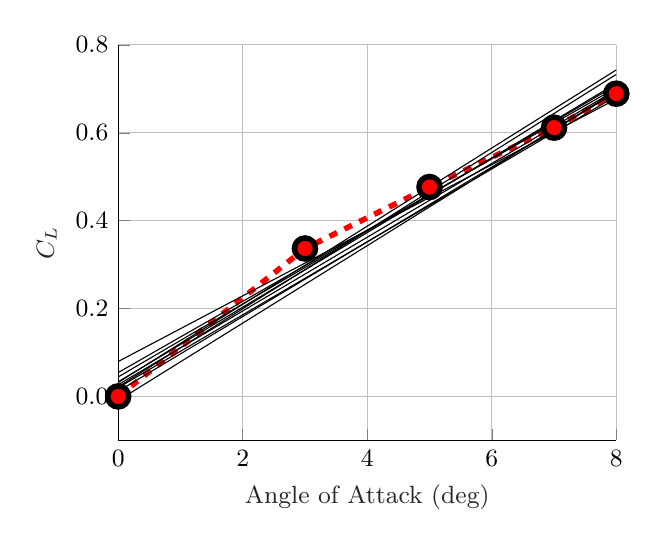
\begin{tikzpicture}

\begin{axis}[%
width=0.958\fwidth,
height=\fheight,
at={(0\fwidth,0\fheight)},
xmin=0,
xmax=8,
xlabel style={font=\color{white!15!black}\small},
xlabel={Angle of Attack (deg)},
ymin=-0.1,
ymax=0.8,
ylabel style={font=\color{white!15!black}\small},
ylabel={$C_L$},
yticklabel style={
            /pgf/number format/fixed,
            /pgf/number format/precision=1,
            /pgf/number format/fixed zerofill
        },
axis background/.style={fill=white},
axis x line*=bottom,
axis y line*=left,
xmajorgrids,
ymajorgrids,
tick label style={font=\small}
]
\addplot [color=red, dashed, line width=2.0pt, mark size=3.8pt, mark=*, mark options={solid, fill=red, draw=black}, forget plot]
  table[row sep=crcr]{%
0	0\\
3	0.336668611\\
5	0.476583991\\
7	0.611685107\\
8	0.688973236\\
};
\addplot [color=black, forget plot]
  table[row sep=crcr]{%
0	0.0542183910320263\\
3	0.297423125663281\\
5	0.459559615417451\\
7	0.621696105171621\\
8	0.702764350048706\\
};
\addplot [color=black, forget plot]
  table[row sep=crcr]{%
0	0.0217583489696848\\
3	0.288447267891223\\
5	0.466239880505581\\
7	0.64403249311994\\
8	0.732928799427119\\
};
\addplot [color=black, forget plot]
  table[row sep=crcr]{%
0	0.0317886771948997\\
3	0.298550641432827\\
5	0.476391950924779\\
7	0.654233260416731\\
8	0.743153915162707\\
};
\addplot [color=black, forget plot]
  table[row sep=crcr]{%
0	0.0266342703142139\\
3	0.27839844393406\\
5	0.44624122634729\\
7	0.61408400876052\\
8	0.698005399967136\\
};
\addplot [color=black, forget plot]
  table[row sep=crcr]{%
0	0.0332150201637679\\
3	0.287963323582276\\
5	0.457795525861281\\
7	0.627627728140287\\
8	0.71254382927979\\
};
\addplot [color=black, forget plot]
  table[row sep=crcr]{%
0	0.01970199639153\\
3	0.268719509864089\\
5	0.434731185512461\\
7	0.600742861160833\\
8	0.68374869898502\\
};
\addplot [color=black, forget plot]
  table[row sep=crcr]{%
0	0.0794439380630236\\
3	0.303470366562141\\
5	0.452821318894886\\
7	0.602172271227631\\
8	0.676847747394003\\
};
\addplot [color=black, forget plot]
  table[row sep=crcr]{%
0	0.0116694144989497\\
3	0.266820896484215\\
5	0.436921884474392\\
7	0.607022872464569\\
8	0.692073366459658\\
};
\addplot [color=black, forget plot]
  table[row sep=crcr]{%
0	-0.00942489875180126\\
3	0.25500232031907\\
5	0.431287133032984\\
7	0.607571945746898\\
8	0.695714352103855\\
};
\addplot [color=black, forget plot]
  table[row sep=crcr]{%
0	0.0442983092486217\\
3	0.29339610539177\\
5	0.459461302820535\\
7	0.625526500249301\\
8	0.708559098963684\\
};
\end{axis}
\end{tikzpicture}%
    \caption{Monte Carlo simulation of uncorrected coefficient of lift data.}
    \label{fig:Incorrect}
\end{figure}

\begin{figure}[H]
    \centering
    % This file was created by matlab2tikz.
%
%The latest updates can be retrieved from
%  http://www.mathworks.com/matlabcentral/fileexchange/22022-matlab2tikz-matlab2tikz
%where you can also make suggestions and rate matlab2tikz.
%
\definecolor{mycolor1}{rgb}{0.65098,0.65098,0.65098}
%
\begin{tikzpicture}

\begin{axis}[%
width=0.958\fwidth,
height=\fheight,
at={(0\fwidth,0\fheight)},
xmin=-1,
xmax=8,
xlabel style={font=\color{white!15!black}\small},
xlabel={Angle of Attack (deg)},
ymin=-0.1,
ymax=0.8,
ylabel style={font=\color{white!15!black}\small},
ylabel={$C_L$},
yticklabel style={
            /pgf/number format/fixed,
            /pgf/number format/precision=1,
            /pgf/number format/fixed zerofill
        },
axis background/.style={fill=white},
axis x line*=bottom,
axis y line*=left,
xmajorgrids,
ymajorgrids,
tick label style={font=\small}
]
\addplot [color=red, dashed, line width=2.0pt, mark size=3pt, mark=*, mark options={solid, fill=mycolor1, draw=black}, forget plot]
  table[row sep=crcr]{%
0	0\\
3	0.32308476\\
5	0.457573009\\
7	0.586722313\\
8	0.658572369\\
};
\addplot [color=black, forget plot]
  table[row sep=crcr]{%
0	0.00797574649264981\\
3	0.271998851745137\\
5	0.448014255246795\\
7	0.624029658748454\\
8	0.712037360499283\\
};
\addplot [color=black, forget plot]
  table[row sep=crcr]{%
0	0.0345902279959458\\
3	0.262537790369622\\
5	0.414502831952073\\
7	0.566467873534524\\
8	0.64245039432575\\
};
\addplot [color=black, forget plot]
  table[row sep=crcr]{%
0	0.0521843651766917\\
3	0.270461898216285\\
5	0.415980253576013\\
7	0.561498608935742\\
8	0.634257786615607\\
};
\addplot [color=black, forget plot]
  table[row sep=crcr]{%
0	0.101771172346943\\
3	0.3070868341458\\
5	0.443963942011705\\
7	0.58084104987761\\
8	0.649279603810563\\
};
\addplot [color=black, forget plot]
  table[row sep=crcr]{%
0	0.0271684666589282\\
3	0.275087973540868\\
5	0.440367644795495\\
7	0.605647316050121\\
8	0.688287151677434\\
};
\addplot [color=black, forget plot]
  table[row sep=crcr]{%
0	0.0395087021792015\\
3	0.275025550432307\\
5	0.432036782601044\\
7	0.589048014769781\\
8	0.667553630854149\\
};
\addplot [color=black, forget plot]
  table[row sep=crcr]{%
0	-0.00201694799454762\\
3	0.258411944468262\\
5	0.432031206110134\\
7	0.605650467752007\\
8	0.692460098572944\\
};
\addplot [color=black, forget plot]
  table[row sep=crcr]{%
0	-0.0175728372085651\\
3	0.252632460674605\\
5	0.432769325930052\\
7	0.612906191185499\\
8	0.702974623813222\\
};
\addplot [color=black, forget plot]
  table[row sep=crcr]{%
0	0.0409477997462568\\
3	0.280476292277049\\
5	0.440161953964244\\
7	0.599847615651439\\
8	0.679690446495037\\
};
\addplot [color=black, forget plot]
  table[row sep=crcr]{%
0	0.0154790863496489\\
3	0.261823789336333\\
5	0.426053591327455\\
7	0.590283393318577\\
8	0.672398294314139\\
};
\end{axis}
\end{tikzpicture}%
    \caption{Monte Carlo simulation of corrected coefficient of lift data.}
    \label{fig:Correct}
\end{figure}

\noindent
This lab report was typeset using \LaTeX.

\begin{thebibliography}{99}
    \bibitem{lab5r1} Abbitt, J. D., ``Wind Tunnel Corrections - Part 1,'' \textit{University of Florida} [PowerPoint slides], URL: \url{https://ufl.instructure.com/courses/480244/files/77543932/}, 2023.
    \bibitem{shape} Barlow, J. B., Rae, W. H., Pope, A., ``Boundary Corrections I: Basics and Two-Dimensional Cases'', \textit{Low-Speed Wind Tunnel Testing}, 3rd ed., Wiley, New York, 1999, p. 353.
    \bibitem{lab3} Borg., A., Lam., B., Latzko, A., ``Characterizing the Wake Region of a Smooth Cylinder,'' \textit{University of Florida}, 2023.
    \bibitem{ports} Abbitt, J. D., ``Airfoil Geometries,'' \textit{University of Florida} [PDF], URL: \url{https://ufl.instructure.com/courses/480244/files/77543942/}, 2023.
    \bibitem{AirfoilEq} Jacobs, E. N., Ward, K. E., Pinkerton, R. M., ``The Characteristics of 78 Related Airfoil Sections from Tests in the Variable-Density Wind Tunnel,'' NACA Report No. 460, Jan 1933.
    \bibitem{XFOIL} Barrett, R., and Ning, A., ``Comparison of Airfoil Precomputational Analysis Methods for Optimization of Wind Turbine Blades'', \textit{IEEE Transactions on Sustainable Energy}, Vol. 7, No. 3, Jul. 2016, pp. 1081--1088.
    \bibitem{Symmetrical} Flandro, G. A., McMahon, H. M., Roach, R. L., ``Two-Dimensional Airfoils'', \textit{Basic Aerodynamics: Incompressible Flow}, Cambridge Univ. Press, New York, 2012, p. 194.
    \bibitem{HeatTrans} Bergman, T. L., and Lavine, A. S., ``Appendix A: Thermophysical Properties of Matter,'' \textit{Fundamentals of Heat and Mass Transfer}, Wiley, Hoboken, NJ, 2017, p. 911.
    \bibitem{MoMLecture} Ridgeway, S., ``MOM\_lab Uncertainty basics w tension,'' \textit{University of Florida} [PowerPoint slides], URL: \url{https://ufl.instructure.com/courses/447927/files/65674680}, 2022.
    \bibitem{errorprop} Ku, H. H., ``Notes on the Use of Propagation of Error Formulas'', \textit{Journal of Research of the National Bureau of Standards}, Vol. 70C, No. 4, 27 May 1966, pp. 263--273.
\end{thebibliography}

\end{document}